% complie with xelatex
\documentclass[hyperref, twocolumn, 9pt]{extarticle}
\usepackage{extsizes}
\usepackage[a4paper, landscape, top=1.0cm, bottom=1.5cm, left=1.5cm, right=1.5cm]{geometry}
\usepackage{ctex}
\usepackage{listings}
\usepackage{lipsum}
\usepackage{xcolor}
\usepackage{fontspec}
\usepackage{hyperref}
\usepackage{amsmath}
\usepackage{amssymb}
\usepackage{graphicx}

\hypersetup{hidelinks}
\setlength{\columnsep}{1cm}
\setlength{\parindent}{0pt}
\linespread{1}
\lstset{
    basicstyle=\fontspec{Consolas}\small, % 基本字体样式
    keywordstyle=\bfseries\color{purple}\fontseries{b}\selectfont, % 关键字颜色
    commentstyle=\color{green!30!gray}, % 注释颜色
    stringstyle=\itshape\color{blue}, % 字符串颜色
    numbers=left, % 显示行号
    numberstyle=\tiny\color{gray}, % 行号样式
    breaklines=true, % 自动换行
    tabsize=4, % 制表符宽度
    extendedchars=true, % 支持非 ASCII 字符（中文可能还需额外设置）
    morekeywords={constexpr, nullptr, override}, % 自定义关键
}

\begin{document}

\begin{titlepage}
    \centering
    \vspace*{2cm}

    {\fontsize{25pt}{28pt}\bfseries 老司机带带我\par}
    \vspace{0.5cm}
    {\fontsize{20pt}{17pt}\rm old driver take me\par}

    \vspace{10cm}

    {\fontsize{15pt}{17pt}\rm 吴子健 \quad 林宇煌 \quad 朱芝毅 \par}
    \vspace{0.2cm}

    {\fontsize{15pt}{17pt}\rm \today}
    \vspace{2cm}
\end{titlepage}

\tableofcontents

\section{基本算法与杂项}

蔡勒公式
\[
w=\left(y+\left[{\frac {y}{4}}\right]+\left[{\frac {c}{4}}\right]-2c+\left[{\frac {26(m+1)}{10}}\right]+d-1\right){\bmod {7}}
\]
或
\[
w=\left(y+\left[{\frac {y}{4}}\right]+\left[{\frac {c}{4}}\right]-2c+2m+\left[{\frac {3(m+1)}{5}}\right]+d+1\right){\bmod {7}}
\]

\subsection{三分}

A. 整数域三分，求凸函数的极小值
\begin{lstlisting}[language = C++]
ll ternary_search(ll l,ll r){
	ll lmid, rmid;
	while(r-l > 2){
		lmid = l+(r-l)/3;
		rmid = r-(r-l)/3;
		if(check(lmid) <= check(rmid)) r = rmid;
		else l = lmid; 
	}
	return min(check(l), min(check(l+1), check(l+2)));
} 
\end{lstlisting}

B. 实数域三分，求凹函数的极大值
\begin{lstlisting}[language = C++]
double ternary_search(double l, double r){
	double mid, lmid, rmid;
	while(r-l > eps){
        mid = l+(r-l)/2;
        lmid = mid-eps, rmid = mid+eps;
        if(f(lmid) > f(rmid)) r = mid;
        else l = mid;
    }
	return f(l);
}
\end{lstlisting}

\subsection{对拍}

\begin{lstlisting}[language=C++]
// Windows
void solve() {
    system("g++ -std=c++23 data.cpp -o data.exe");
    system("g++ -std=c++23 std.cpp -o std.exe");
    system("g++ -std=c++23 solve.cpp -o solve.exe");
    int t = 0;
    while (true) {
        cout << "test" << ++t << ": ";
        system("data.exe > data.in");
        system("std.exe < data.in > std.ans");
        system("solve.exe < data.in > solve.ans");
        if (system("fc std.ans solve.ans > diff.log")) {
            cout << "WA" << endl;
            system("type data.in");
            system("type std.ans");
            system("type solve.ans");
            system("pause");
            break;
        }
        cout << "AC" << endl;
    }
}
// Linux
void solve() {
    system("rm data; rm solve; rm std; make data && make solve && make std");
    int t = 0;
    while (true) {
        cout << "test" << ++t << ": ";
        system("./data > in");
        system("./solve < in > solve.ans");
        system("./std < in > std.ans");
        if (system("diff solve.ans std.ans")) {
            cout << "WA" << endl;
            system("pause");
            break;
        }
        cout << "AC" << endl;
    }
}
\end{lstlisting}

\subsection{高精度}

\begin{lstlisting}[language=C++]
struct BigInteger {
    vector<int> digits;
    bool isNegative = false;

    BigInteger(int num) {
        if (num < 0) {
            isNegative = true;
            num = -num;
        }
        do {
            digits.push_back(num % 10);
            num /= 10;
        } while (num > 0);
        removeLeadingZeros();
    }
    BigInteger(const string& num = "0") {
        if (num[0] == '-') {
            isNegative = true;
            for (int i = num.size() - 1; i > 0; i--) {
                digits.push_back(num[i] - '0');
            }
        } else {
            for (int i = num.size() - 1; i >= 0; i--) {
                digits.push_back(num[i] - '0');
            }
        }
        removeLeadingZeros();
    }

    BigInteger operator+(const BigInteger& other) const {
        if (isNegative == other.isNegative) {
            BigInteger result;
            result.isNegative = isNegative;
            int carry = 0;
            for (size_t i = 0; i < max(digits.size(), other.digits.size()) || carry; i++) {
                if (i < digits.size()) carry += digits[i];
                if (i < other.digits.size()) carry += other.digits[i];
                result.digits.push_back(carry % 10);
                carry /= 10;
            }
            result.removeLeadingZeros();
            return result;
        }
        return isNegative ? (other - (-*this)) : (*this - (-other));
    }
    BigInteger operator-(const BigInteger& other) const {
        if (isNegative == other.isNegative) {
            if (isNegative) return (-other) - (-*this);
            if (*this < other) return -(other - *this);
            BigInteger result;
            int borrow = 0;
            for (size_t i = 0; i < digits.size(); ++i) {
                int diff = digits[i] - borrow;
                if (i < other.digits.size()) diff -= other.digits[i];
                if (diff < 0) {
                    diff += 10;
                    borrow = 1;
                } else {
                    borrow = 0;
                }
                result.digits.push_back(diff);
            }
            result.removeLeadingZeros();
            return result;
        }
        return isNegative ? -(-*this + other) : (*this + (-other));
    }
    BigInteger operator*(const BigInteger& other) const {
        BigInteger result;
        result.digits.resize(digits.size() + other.digits.size());
        for (size_t i = 0; i < digits.size(); ++i) {
            int carry = 0;
            for (size_t j = 0; j < other.digits.size() || carry; ++j) {
                int cur = result.digits[i + j] + digits[i] * (j < other.digits.size() ? other.digits[j] : 0) + carry;
                result.digits[i + j] = cur % 10;
                carry = cur / 10;
            }
        }
        result.isNegative = (isNegative != other.isNegative);
        result.removeLeadingZeros();
        return result;
    }
    BigInteger operator/(int divisor) const {
        if (divisor == 0) {
            throw runtime_error("Division by zero");
        }

        bool resultNegative = (isNegative ^ (divisor < 0));
        BigInteger dividend = *this;
        dividend.isNegative = false;
        divisor = abs(divisor);
        if (dividend.digits[0] == 0 && dividend.digits.size() == 1) {
            return BigInteger("0");
        }
        string quotientStr;
        int remainder = 0;
        for (int i = dividend.digits.size() - 1; i >= 0; i--) {
            remainder = remainder * 10 + dividend.digits[i];
            int q = remainder / divisor;
            remainder %= divisor;
            quotientStr += to_string(q);
        }
        size_t firstNonZero = 0;
        while (firstNonZero < quotientStr.size() && quotientStr[firstNonZero] == '0') {
            firstNonZero++;
        }
        quotientStr = (firstNonZero == quotientStr.size()) ? "0" : quotientStr.substr(firstNonZero);
        if (resultNegative && remainder != 0) {
            BigInteger temp(quotientStr);
            temp = temp + BigInteger("1"); // 正数加 1，转为负数后即向下取整
            temp.isNegative = true;
            return temp;
        }
        BigInteger quotient(quotientStr);
        quotient.isNegative = resultNegative;
        return quotient;
    }
    bool operator==(const BigInteger& other) const {
        if (isNegative != other.isNegative) {
            return false;
        }
        if (digits.size() != other.digits.size()) {
            return false;
        }
        for (size_t i = 0; i < digits.size(); ++i) {
            if (digits[i] != other.digits[i]) {
                return false;
            }
        }
        return true;
    }
    bool operator>(const BigInteger& other) const {
        if (isNegative != other.isNegative) {
            return isNegative;
        }
        if (digits.size() != other.digits.size()) {
            return (digits.size() > other.digits.size()) ^ isNegative;
        }
        for (int i = digits.size() - 1; i >= 0; i--) {
            if (digits[i] != other.digits[i]) {
                return (digits[i] > other.digits[i]) ^ isNegative;
            }
        }
        return false;
    }
    bool operator<(const BigInteger& other) const {
        if (isNegative != other.isNegative) {
            return isNegative;
        }
        if (digits.size() != other.digits.size()) {
            return (digits.size() < other.digits.size()) ^ isNegative;
        }
        for (int i = digits.size() - 1; i >= 0; i--) {
            if (digits[i] != other.digits[i]) {
                return (digits[i] < other.digits[i]) ^ isNegative;
            }
        }
        return false;
    }
    BigInteger operator-() const {
        BigInteger result = *this;
        result.isNegative = !isNegative;
        return result;
    }
    void removeLeadingZeros() {
        while (digits.size() > 1 && digits.back() == 0) {
            digits.pop_back();
        }
        if (digits.size() == 1 && digits[0] == 0) {
            isNegative = false;
        }
    }
    friend istream& operator>>(istream& is, BigInteger& num) {
        string input;
        is >> input;
        num = BigInteger(input);
        return is;
    }
    friend ostream& operator<<(ostream& os, const BigInteger& num) {
        if (num.isNegative && !(num.digits.size() == 1 && num.digits[0] == 0)) {
            os << '-';
        }
        for (int i = num.digits.size() - 1; i >= 0; i--) {
            os << num.digits[i];
        }
        return os;
    }
};
\end{lstlisting}

\subsection{日期类}

\begin{lstlisting}[language=C++]
int daysInM[13] = {0, 31, 28, 31, 30, 31, 30, 31, 31, 30, 31, 30, 31};
int daysBeforeM[13] = {0, 0, 31, 59, 90, 120, 151, 181, 212, 243, 273, 304, 334};
bool isLeapYear(int year) {
    return year % 400 == 0 || year % 4 == 0 && year % 100 != 0;
}
int daysInMonth(int year, int month) {
    return daysInM[month] + (month == 2 ? isLeapYear(year) : 0);
}
struct Date {
    int year, month, day;
    bool isLeap;
    int daysFromAD; // 公元1年1月1日(星期一)到当前日期总天数，算上了1582.10.5~14
    int weekDay;
    Date(int year_, int month_, int day_) : year(year_), month(month_), day(day_) {
        isLeap = isLeapYear(year);
        int y = year - 1;
        daysFromAD = y * 365 + y / 4 - y / 100 + y / 400 + daysBeforeM[month] + day - 1;
        if (isLeap && month > 2) {
            daysFromAD++;
        }
        weekDay = (daysFromAD + 1) % 7;
    }
    Date(int days) {
        daysFromAD = days;
        weekDay = (daysFromAD + 1) % 7;
        year = days / 365 + 1;
        int d;
        while (year > 1) {
            int y = year - 1;
            d = y * 365 + y / 4 - y / 100 + y / 400;
            if (d <= days) {
                break;
            }
            year--;
        }
        isLeap = isLeapYear(year);
        d = days - d + 1;
        month = 1;
        while (month < 12) {
            int dIM = daysInMonth(year, month);
            if (d <= dIM) {
                break;
            }
            d -= dIM;
            month++;
        }
        day = d;
    }
    void print() {
        cout << year << "/" << month << "/" << day << ", " << weekDay << ", " << daysFromAD << "\n";
    }
};
int daysBetween(const Date &u, const Date &v) {
    return abs(u.daysFromAD - v.daysFromAD);
}
\end{lstlisting}

\subsection{取模类}

\begin{lstlisting}[language=C++]
using ll = long long;

template<typename T>
T fpow(T x, int y){
    T res = 1;
    for(; y; y >>= 1){
        if(y&1) res *= x;
        x *= x;
    }
    return res;
}

template<int M>
struct Mint{
    ll val;
    Mint(): val(0) {}
    Mint(ll x): val((x%M+M)%M) {}
    Mint(const Mint<M> &t): val(t.val) {}
    Mint inv() const {return fpow<Mint<M>>(*this, M-2);}
    Mint inv() {return fpow<Mint<M>>(*this, M-2);}
    Mint<M>& operator = (const ll &t){
        val = (t%M+M)%M;
        return *this;
    }
    Mint<M>& operator += (const Mint<M> &t){
        val += t.val;
        if(val >= M) val -= M;
        return *this;
    }
    Mint<M>& operator -= (const Mint<M> &t){
        val -= t.val;
        if(val < 0) val += M;
        return *this;
    }
    Mint<M>& operator *= (const Mint<M> &t){
        val = (val*t.val)%M;
        return *this;
    }
    Mint<M>& operator /= (const Mint<M> &t){
        (*this) *= t.inv();
        return *this;
    }
    Mint<M> operator + (const Mint<M> &t){
        Mint<M> u(*this);
        return u += t;
    }
    Mint<M> operator - (const Mint<M> &t){
        Mint<M> u(*this);
        return u -= t;
    }
    Mint<M> operator * (const Mint<M> &t){
        Mint<M> u(*this);
        return u *= t;
    }
    Mint<M> operator / (const Mint<M> &t){
        Mint<M> u(*this);
        return u /= t;;
    }
    bool operator != (const Mint<M> &t) {return t.val != val;}
    bool operator != (ll &t) {return t != val;}
    bool operator == (const Mint<M> &t) {return t.val == val;}
    bool operator == (ll &t) {return t == val;}
    friend ostream& operator << (ostream &os, const Mint<M> &t){
        os << t.val;
        return os;
    }
    friend istream& operator >> (istream &is, Mint<M> &t){
        ll num; is >> num;
        t = num;
        return is;
    }
};
\end{lstlisting}






\section{数据结构}

\subsection{线段树整合}

\begin{lstlisting}[language=C++]
struct Tag {
    int x;
    void apply(const Tag &t) {}
};

struct Info {
    int l, r;
    void apply(const Tag &t) {}
};
Info operator+(const Info &u, const Info &v) {
    Info res;
    res.l = u.l;
    res.r = v.r;
    return res;
}

struct LazySegmentTree {
    int n;
    vector<Info> info;
    vector<Tag> tag;
    LazySegmentTree(int n_, Info v_ = Info()) {
        init(n_, v_);
    }
    LazySegmentTree(const vector<Info> &init_) {
        init(init_);
    }
    void init(int n_, Info v_ = Info()) {
        init(vector(n_, v_)); // seg(n + 1)
    }
    void init(const vector<Info> init_) {
        n = init_.size() - 1; // init_ 大小为 n + 1
        info.assign(4 << __lg(n), Info());
        tag.assign(4 << __lg(n), Tag());
        function<void(int, int, int)> build = [&](int p, int l, int r) {
            if (l == r) {
                info[p] = init_[l];
                info[p].l = l;
                info[p].r = r;

                return;
            }
            int m = l + r >> 1;
            build(p << 1, l, m);
            build(p << 1 | 1, m + 1, r);
            pull(p);
        };
        build(1, 1, n);
    }
    void pull(int p) {
        info[p] = info[p << 1] + info[p << 1 | 1];
    }
    void apply(int p, int l, int r, const Tag &v) {
        info[p].apply(v);
        tag[p].apply(v);
    }
    void push(int p, int l, int r) {
        int m = l + r >> 1;
        apply(p << 1, l, m, tag[p]);
        apply(p << 1 | 1, m + 1, r, tag[p]);
        tag[p] = Tag();
    }
    Info rangeQuery(int p, int l, int r, int x, int y) {
        if (x <= l && r <= y) {
            return info[p];
        }
        push(p, l, r);
        int m = l + r >> 1;
        if (y <= m) {
            return rangeQuery(p << 1, l, m, x, y);
        } else if (x >= m + 1) {
            return rangeQuery(p << 1 | 1, m + 1, r, x, y);
        } else {
            return rangeQuery(p << 1, l, m, x, y) + rangeQuery(p << 1 | 1, m + 1, r, x, y);
        }
    }
    Info rangeQuery(int l, int r) {
        return rangeQuery(1, 1, n, l, r);
    }
    void rangeModify(int p, int l, int r, int x, int y, const Tag &v) {
        if (x <= l && r <= y) {
            apply(p, l, r, v);
            return;
        }
        push(p, l, r);
        int m = l + r >> 1;
        if (y <= m) {
            rangeModify(p << 1, l, m, x, y, v);
        } else if (x >= m + 1) {
            rangeModify(p << 1 | 1, m + 1, r, x, y, v);
        } else {
            rangeModify(p << 1, l, m, x, y, v);
            rangeModify(p << 1 | 1, m + 1, r, x, y, v);
        }
        pull(p);
    }
    void rangeModify(int l, int r, const Tag &v) {
        rangeModify(1, 1, n, l, r, v);
    }
    void modify(int p, int l, int r, int x, const Info &v) {
        if (l == r) {
            info[p] = v;
            return;
        }
        push(p, l, r);
        int m = l + r >> 1;
        if (x <= m) {
            modify(p << 1, l, m, x, v);
        } else {
            modify(p << 1 | 1, m + 1, r, x, v);
        }
        pull(p);
    }
    void modify(int x, const Info &v) {
        modify(1, 1, n, x, v);
    }    
    template<class F>
    int findFirst(int p, int l, int r, int x, int y, F &&pred) {
        if (y < l || r < x) {
            return -1;
        }
        if (x <= l && r <= y && !pred(info[p])) {
            return -1;
        }
        if (l == r) {
            return l;
        }
        push(p, l, r);
        int m = l + r >> 1;
        int res = findFirst(p << 1, l, m, x, y, pred);
        if (res == -1) {
            res = findFirst(p << 1 | 1, m + 1, r, x, y, pred);
        }
        return res;
    }
    template<class F>
    int findFirst(int l, int r, F &&pred) {
        return findFirst(1, 1, n, l, r, pred);
    }
    template<class F>
    int findLast(int p, int l, int r, int x, int y, F &&pred) {
        if (y < l || r < x) {
            return -1;
        }
        if (x <= l && r <= y && !pred(info[p])) {
            return -1;
        }
        if (l == r) {
            return l;
        }
        push(p, l, r);
        int m = l + r >> 1;
        int res = findLast(p << 1 | 1, m + 1, r, x, y, pred);
        if (res == -1) {
            res = findLast(p << 1, l, m, x, y, pred);
        }
        return res;
    }
    template<class F>
    int findLast(int l, int r, F &&pred) {
        return findLast(1, 1, n, l, r, pred);
    }
}
// by lyh
\end{lstlisting}

\subsection{可持久化线段树}

维护历史区间最大值

\begin{lstlisting}[language=C++]
struct node{
    int lc, rc, dat;
}tr[M];

int build(int l, int r){
    int p = ++tot;
    if(l == r){
        tr[p].dat = a[l];
        return p;
    }
    int mid = (l+r)>>1;
    tr[p].lc = build(l, mid);
    tr[p].rc = build(mid+1, r);
    tr[p].dat = max(tr[tr[p].lc].dat, tr[tr[p].rc].dat);
    return p;
}

int insert(int k, int l, int r, int pos, int val){
    int p = ++tot;
    tr[p] = tr[k];
    if(l == r){
        tr[p].dat = val;
        return p;
    }
    int mid = (l+r)>>1;
    if(mid >= pos) tr[p].lc = insert(tr[k].lc, l, mid, pos, val);
    else tr[p].rc = insert(tr[k].rc, mid+1, r, pos, val);
    tr[p].dat = max(tr[tr[p].lc].dat, tr[tr[p].rc].dat);
    return p;
}

int query(int k, int l, int r, int L, int R){
    int res = -2e9;
    if(l >= L && r <= R) return tr[k].dat;
    int mid = (l+r)>>1;
    if(mid >= L) res = max(res, query(tr[k].lc, l, mid, L, R));
    if(mid < R) res = max(res, query(tr[k].rc, mid+1, r, L, R));
    return res; 
}
\end{lstlisting}

查询区间第 $k$ 小值（静态）

\begin{lstlisting}[language=C++]
#include<bits/stdc++.h>
using namespace std;

const int N = 2e5+10;
int n, m, tot, num;
int a[N], b[N], c[N], root[N];

struct node{
    int lc, rc, dat;
}tr[N<<5];

int build(int l, int r){
    int p = ++tot;
    if(l == r){
        tr[p].dat = 0;
        return p;
    }
    int mid = (l+r)>>1;
    tr[p].lc = build(l, mid);
    tr[p].rc = build(mid+1, r);
    tr[p].dat = tr[tr[p].lc].dat+tr[tr[p].rc].dat;
    return p;
}

int change(int k, int l, int r, int pos, int val){
    int p = ++tot;
    tr[p] = tr[k];
    if(l == r){
        tr[p].dat += val;
        return p;
    }
    int mid = (l+r)>>1;
    if(mid >= pos) tr[p].lc = change(tr[k].lc, l, mid, pos, val);
    else tr[p].rc = change(tr[k].rc, mid+1, r, pos, val);
    tr[p].dat = tr[tr[p].lc].dat+tr[tr[p].rc].dat;
    return p;
}

int query(int i, int j, int l, int r, int k){
    if(l == r) return l;
    int mid = (l+r)>>1;
    int cntl = tr[tr[j].lc].dat-tr[tr[i].lc].dat;
    if(cntl >= k) return query(tr[i].lc, tr[j].lc, l, mid, k);
    else return query(tr[i].rc, tr[j].rc, mid+1, r, k-cntl);
}

int Q(int x) {return lower_bound(c+1, c+num+1, x)-c;}

void discrete(){
    for(int i = 1; i <= n; i++) b[i] = a[i];
    sort(b+1, b+n+1);
    b[0] = -1;
    num = 0;
    for(int i = 1; i <= n; i++)
        if(b[i] != b[i-1]) c[++num] = b[i];
    for(int i = 1; i <= n; i++)
        a[i] = Q(a[i]);
}

int main(){
    ios::sync_with_stdio(0);
    cin.tie(0);
    cin >> n >> m;
    for(int i = 1; i <= n; i++)
        cin >> a[i];
    discrete();
    root[0] = build(1, num);
    for(int i = 1; i <= n; i++)
        root[i] = change(root[i-1], 1, num, a[i], 1);
    for(int i = 1; i <= m; i++){
        int l, r, k;
        cin >> l >> r >> k;
        int id = query(root[l-1], root[r], 1, num, k);
        cout << c[id] << endl;
    }
    return 0;
}
\end{lstlisting}

\subsection{可持久化并查集}

\subsection{李超线段树}

\begin{lstlisting}[language=C++]
using ll = long long;
using pii = pair<int, int>;
using pdi = pair<double, int>;
const int N = 1e5+10, modx = 39989, mody = 1e9+7;
const double eps = 1e-9;
struct line{
    double k, b;
    line(double _k = 0, double _b = 0): k(_k), b(_b) {}
}l[N];
int n, tot, tr[N<<2];

line get_line(double x1, double y1, double x2, double y2){
    if(x1 == x2) return line(0, max(y1, y2));
    return line((y1-y2)/(x1-x2), (x1*y2-x2*y1)/(x1-x2));
}

double calc(int i, ll x){
    return l[i].k*x+l[i].b;
}

int cmp(double x, double y){
    if(x-y > eps) return 1;
    if(y-x > eps) return -1;
    return 0;
}

pdi pmax(pdi a, pdi b){
    if(cmp(a.first, b.first) == 1) return a;
    if(!cmp(a.first, b.first))
        return a.second < b.second ? a : b;
    return b;
}

void update(int k, int l, int r, int u){
    int &v = tr[k], mid = (l+r)>>1;
    int cmid = cmp(calc(u, mid), calc(v, mid));
    if(cmid == 1 || (!cmid && u < v)) swap(u, v);
    int cl = cmp(calc(u, l), calc(v, l)), rl = cmp(calc(u, r), calc(v, r));
    if(cl == 1 || (!cl && u < v)) update(k<<1, l, mid, u);
    if(rl == 1 || (!rl && u < v)) update((k<<1)|1, mid+1, r, u);
}

void insert(int k, int l, int r, int L, int R, int u){
    if(l >= L && r <= R){
        update(k, l, r, u);
        return ;
    }
    int mid = (l+r)>>1;
    if(mid >= L) insert(k<<1, l, mid, L, R, u);
    if(mid < R) insert((k<<1)|1, mid+1, r, L, R, u);
}

pdi query(int k, int l, int r, ll x){
    int mid = (l+r)>>1;
    pdi res = {calc(tr[k], x), tr[k]};
    if(l == r) return res;
    if(x <= mid) res = pmax(res, query(k<<1, l, mid, x));
    if(x > mid) res = pmax(res, query((k<<1)|1, mid+1, r, x)); 
    return res;
}
\end{lstlisting}


\subsection{树状数组求第 $k$ 大}

\begin{lstlisting}[language=C++]

template<class T>
struct Fenwick {
    int n;
    vector<T> f;
    Fenwick(int n) {
        init(n);
    }
    void init(int n) {
        this->n = n;
        f.assign(n, 0);
    }
    void add(int x, T k) {
        assert(x > 0);
        for (; x < n; x += x & -x) {
            f[x] += k;
        }
    }
    T pre(int x) {
        assert(x < n);
        T res {};
        for (; x; x -= x & -x) {
            res += f[x];
        }
        return res;
    }
    T rangeSum(int l, int r) {
        return pre(r) - pre(l - 1);
    }
    int kth(int k) {
        int x = 0;
        T cur {};
        for (int i = 1 << __lg(n); i; i >>= 1) {
            if (x + i < n && cur + f[x + i] < k) {
                cur += f[x + i];
                x += i;
            }
        }
        return x + 1;
    }
};
\end{lstlisting}

\subsection{笛卡尔树}

每个节点为一对键值 $(k, w)$，其中 $k$ 满足二叉搜索树的性质，$w$ 满足堆的性质，通过单调栈维护右链建树，新的节点插入到右链，将 $w$ 大于该节点的子树作为左子树。

\begin{lstlisting}[language = C++]
// stk 维护笛卡尔树中节点对应到序列中的下标
for (int i = 1; i <= n; i++) {
    int k = top;  // top 表示操作前的栈顶，k 表示当前栈顶
    while(k > 0 && w[stk[k]] > w[i]) k--;  // 维护右链上的节点
    if(k) rs[stk[k]] = i;  // 栈顶元素.右儿子 := 当前元素
    if(k < top) ls[i] = stk[k + 1]; 
    // 当前元素.左儿子 := 上一个被弹出的元素  
    stk[++k] = i; // 当前元素入栈
    top = k;
}
\end{lstlisting}

\subsection{pbds tree}

\begin{lstlisting}[language=C++]
#include <bits/extc++.h>
using namespace __gnu_pbds;
using pbds_tree = tree<array<int, 2>, null_type, less<>, rb_tree_tag, tree_order_statistics_node_update>;

void solve() {
    int idx = 0; // 有重复元素，要设置唯一索引
    pbds_tree t;
    while (q--) {
        if (o == 1) {
            // 插入
            t.insert({x, idx++});
        } else if (o == 2) {
            // 删除
            auto it = t.lower_bound({x, 0});
            if (it != t.end() && (*it)[0] == x) {
                t.erase(it);
            }
        } else if (o == 3) {
            // 排名
            cout << t.order_of_key({x, 0}) + 1 << "\n"; 
        } else if (o == 4) {
            // 第 x 大，find_by_order 是 0-based，要查 x - 1
            cout << (*t.find_by_order(x - 1))[0] << "\n";
        } else if (o == 5) {
            // 前驱
            cout << (*--t.lower_bound({x, 0}))[0] << "\n";
        } else {
            // 后继
            cout << (*t.upper_bound({x, idx}))[0] << "\n";
        }
    }
}
\end{lstlisting}

\subsection{pbds pq}

\begin{lstlisting}[language=C++]
using pbds_pq = __gnu_pbds::priority_queue<array<int, 2>, greater<>>;

void solve() {
    int n, m;
    cin >> n >> m;
    
    vector<pbds_pq> pq(n + 1);
    for (int i = 1; i <= n; i++) {
        int x;
        cin >> x;
        pq[i].push({x, i});
    }
    
    vector<bool> del(n + 1);
    DSU dsu(n + 1);

    while (m--) {
        int o;
        cin >> o;
        
        if (o == 1) {
            // 合并第 x 个数和第 y 个数所在的堆
            int x, y;
            cin >> x >> y;
            
            int fx = dsu.find(x);
            int fy = dsu.find(y);
            if (del[x] || del[y] || fx == fy) {
                continue;
            }
            if (pq[fx].size() < pq[fy].size()) {
                swap(fx, fy);
            }
            pq[fx].join(pq[fy]);
            dsu.merge(fx, fy);

        } else {
            // 删除第 x 个数所在堆的堆顶
            int x;
            cin >> x;

            if (del[x]) {
                cout << "-1\n";
            } else {
                x = dsu.find(x);

                auto [val, id] = pq[x].top();
                pq[x].pop();

                del[id] = true;
                cout << val << "\n";
            }
        }
    }
}
\end{lstlisting}

\subsection{树状数组套线段树}

\begin{lstlisting}[language=C++]
int Y = 2e5;
struct Node {
    int l = 0, r = 0;
    int ls = 0, rs = 0;
    int sum = 0, add = 0;
};
vector<Node> in;
int newNode(int l, int r) {
    Node node;
    node.l = l;
    node.r = r;
    in.push_back(node);
    return in.size() - 1;
}
void push(int p) {
    if (in[p].add == 0 || in[p].l == in[p].r) {
        return;
    }
    int m = (in[p].l + in[p].r) >> 1;
    if (!in[p].ls) {
        in[p].ls = newNode(in[p].l, m);
    }
    if (!in[p].rs) {
        in[p].rs = newNode(m + 1, in[p].r);
    }
    in[in[p].ls].sum += (m - in[p].l + 1) * in[p].add;
    in[in[p].ls].add += in[p].add;
    in[in[p].rs].sum += (in[p].r - m) * in[p].add;
    in[in[p].rs].add += in[p].add;
    in[p].add = 0;
}
void pull(int p) {
    in[p].sum = 0;
    if (in[p].ls) {
        in[p].sum += in[in[p].ls].sum;
    }
    if (in[p].rs) {
        in[p].sum += in[in[p].rs].sum;
    }
}
int rangeModify(int p, int l, int r, int yl, int yr, int k) {
    if (yr < l || r < yl) {
        return p;
    }
    if (!p) {
        p = newNode(l, r);
    }
    if (yl <= l && r <= yr) {
        in[p].sum += (r - l + 1) * k;
        in[p].add += k;
        return p;
    }
    push(p);
    int m = (l + r) >> 1;
    in[p].ls = rangeModify(in[p].ls, l, m, yl, yr, k);
    in[p].rs = rangeModify(in[p].rs, m + 1, r, yl, yr, k);
    pull(p);
    return p;
}
int rangeQuery(int p, int yl, int yr) {
    if (!p || yr < in[p].l || in[p].r < yl) {
        return 0;
    }
    if (yl <= in[p].l && in[p].r <= yr) {
        return in[p].sum;
    }
    push(p);
    return rangeQuery(in[p].ls, yl, yr) + rangeQuery(in[p].rs, yl, yr);
}

int X = 2e5;
struct OutNode {
    int inRoot = 0;
};
vector<OutNode> out;
void add(int x, int yl, int yr, int k) {
    assert(x > 0);
    for (; x <= X; x += x & -x) {
        out[x].inRoot = rangeModify(out[x].inRoot, 1, Y, yl, yr, k);
    }
}
int pre(int x, int yl, int yr) {
    assert(x <= X);
    int res = 0;
    for (; x; x -= x & -x) {
        res += rangeQuery(out[x].inRoot, yl, yr);
    }
    return res;
}
\end{lstlisting}

\subsection{ST 表}

\begin{lstlisting}[language=C++]
template<class T>
struct SparseTable {
    using Func = function<T(T, T)>; // lambda
    int n;
    vector<int> log2;
    vector<vector<T>> st;
    Func func;

    SparseTable(const vector<T> &a, Func f) {
        init(a, f);
    }
    void init(const vector<T> &a, Func f) {
        n = a.size();
        func = f;
        int k = __lg(n) + 1;
        log2.assign(n, 0);
        st.assign(n, vector<T>(k));
        for (int i = 2; i < n; i++) {
            log2[i] = log2[i >> 1] + 1;
        }
        for (int i = 1; i < n; i++) {
            st[i][0] = a[i];
        }
        for (int j = 1; j < k; j++) {
            for (int i = 1; i + (1 << j) - 1 < n; i++) {
                st[i][j] = func(st[i][j - 1], st[i + (1 << j - 1)][j - 1]);
            }
        }
    }
    T query(int l, int r) {
        int k = log2[r - l + 1];
        return func(st[l][k], st[r - (1 << k) + 1][k]);
    }
};
// by lyh
\end{lstlisting}

\subsection{XOR Hash}

\begin{lstlisting}[language=C++]
mt19937_64 rng(chrono::steady_clock::now().time_since_epoch().count());
struct XorHash {
    int n;
    vector<int> Base, Xor, Hash;
    XorHash(const vector<int> &a) {
        init(a);
    }
    void init(const vector<int> &a) {
        n = a.size();
        Base.assign(n, 0);
        Xor.assign(n, 0);
        Hash.assign(n, 0);
        for (int i = 1; i < n; i++) {
            Base[i] = rng();
            Xor[i] = Xor[i - 1] ^ Base[i];
        }
        for (int i = 1; i < n; i++) {
            Hash[i] = Hash[i - 1] ^ Base[a[i]];
        }
    }
    bool isPemutation(int l, int r, int s, int t) { // a[l, r]是否是整数[s, t]的排列
        return (Hash[r] ^ Hash[l - 1]) == (Xor[t] ^ Xor[s - 1]);
    }
};
// by lyh
\end{lstlisting}

\subsection{动态图连通性 (线段树分治+可撤销并查集)}

利用线段树对询问进行划分, 每个叶子节点对应一个时间点. 记每条边的存在时间为 $[l, r]$, 将该区间插入线段树中, 线段树的每个节点记录对应时间段内存在的边. 建完树后 dfs 遍历线段树, 访问至叶节点回答询问. 回溯时撤销当前节点对并查集的操作.
\begin{lstlisting}[language=C++]
// LOJ 121
#include<bits/stdc++.h>
using namespace std;

using pii = pair<int, int>;
const int N = 5e3+10, M = 5e5+10;
map<pii, int> mp;
int n, m, ans[M];
pii q[M];
vector<pii> tr[M*20];

struct operation{
    int x, y, s_x;
};
struct DSU{
    int num;
    vector<int> f, s;
    stack<operation> op;
    DSU() {}
    DSU(int sz){
        num = sz;
        f = vector<int> (num+1, 0);
        s = vector<int> (num+1, 1);
        iota(f.begin(), f.end(), 0);
    }
    int find(int x){
        if(f[x] == x) return x;
        return find(f[x]);
    }
    void merge(int x, int y){
        x = find(x); y = find(y);
        if(s[x] > s[y]) swap(x, y);
        op.push({x, y, s[x]});
        if(x != y){
            f[x] = y;
            s[y] += x; s[x] = 0;
        }
    }
    void split(){
        auto [x, y, s_x] = op.top();  
        op.pop();
        if(x == y) return ;
        f[x] = x;
        s[x] = s_x; s[y] -= s_x;
    }
    void back(int x){
        for(int i = 1; i <= x; i++) split();
    }
}g;
void insert(int k, int l, int r, int L, int R, pii e){
    if(l >= L && r <= R){
        tr[k].push_back(e);
        return ;
    }
    int mid = (l+r)>>1;
    if(mid >= L) insert(k<<1, l, mid, L, R, e);
    if(mid < R) insert((k<<1)|1, mid+1, r, L, R, e);
}
void dfs(int k, int l, int r){
    for(auto [x, y]: tr[k])
        g.merge(x, y);
    if(l == r){
        auto [x, y] = q[l];
        if(x == 0 && y == 0) {g.back(tr[k].size()); ans[l] = -1; return ;}
        if(g.find(x) == g.find(y)) ans[l] = 1;
        else ans[l] = 0;
        g.back(tr[k].size());
        return ;
    }
    int mid = (l+r)>>1;
    dfs(k<<1, l, mid);
    dfs((k<<1)|1, mid+1, r);
    g.back(tr[k].size());
}

int main(){
    ios::sync_with_stdio(0);
    cin >> n >> m;
    for(int i = 1; i <= m; i++){
        int op, x, y;
        cin >> op >> x >> y;
        if(x > y) swap(x, y);
        q[i] = {0, 0};
        if(op == 0) mp[{x, y}] = i;
        else if(op == 1){
            insert(1, 1, m, mp[{x, y}], i-1, {x, y});
            mp[{x, y}] = 0;
        }
        else q[i] = {x, y};
    }
    for(auto [e, i]: mp)
        if(i) insert(1, 1, m, i, m, e);
    g = DSU(n);
    dfs(1, 1, m);
    for(int i = 1; i <= m; i++) if(ans[i] != -1){
        if(ans[i]) cout << "Y\n";
        else cout << "N\n";
    }
    return 0;
}
\end{lstlisting}
\section{数学}

\subsection{组合数线性预处理}

\begin{lstlisting}[language=C++]
ll fac[N], inv[N], inv_fac[N];
void binom_init(int n) {
    fac[0] = fac[1] = inv[0] = inv[1] = inv_fac[0] = inv_fac[1] = 1;
    for(int i = 2; i <= n; i++) {
        fac[i] = fac[i - 1] * i % mod;
        inv[i] = (mod - mod / i) * inv[mod % i] % mod;
    }
    for(int i = 2; i <= n; i++) {
        inv_fac[i] = inv_fac[i - 1] * inv[i] % mod;
    }
}
int binom(int n, int m) {
    if (n < 0 || m < 0 || n < m) {
        return 0;
    }
    return fac[n] * inv_fac[m] % mod * inv_fac[n - m] % mod;
}
// by lyh
\end{lstlisting}

\subsection{线性筛}

\begin{lstlisting}[language=C++]
vector<int> primes, minp;
vector<int> phi;
void sieve(int n) {
    minp.assign(n + 1, 0);
    phi.assign(n + 1, 1);
    for (int i = 2; i <= n; i++) {
        if (!minp[i]) {
            primes.push_back(minp[i] = i);
            phi[i] = i - 1;
        }
        for (auto p : primes) {
            if (i * p > n) break;
            minp[i * p] = p;
            phi[i * p] = phi[i] * phi[p];
            if (p == minp[i]) {
                phi[i * p] = phi[i] * p;
                break;
            }
        }
    }
}
// by lyh
\end{lstlisting}

\subsection{扩展欧几里得}

$ax+by=c$ 有解 $\leftrightarrow (a,b)|c$，记 $x_0, y_0$ 为方程 $ax+by=(a,b)$ 的一组解，则原方程的解集为：
\[
    x = \dfrac{c}{g}x_0+k\dfrac{b}{g},\quad y = \dfrac{c}{g}y_0-k\dfrac{a}{g},\quad k\in \mathbb{Z}
\]

\begin{lstlisting}[language = C++]
ll exgcd(ll a, ll b, ll &x, ll &y){
    if(b == 0){
        x = 1; y = 0;
        return a;
    }
    ll g = exgcd(b, a%b, x, y);
    tie(x, y) = make_tuple(y, x-a/b*y);
    return g;
}
\end{lstlisting}

\subsection{高斯消元}

\begin{lstlisting}[language = C++]
double* solve(int n, double a[][N], double b[], int &state){
    state = 1;
    static double x[N];
    int rank = 0;
    memset(x, 0, sizeof(x));
    for(int i = 1; i <= n; i++){
        for(int j = 1; j <= n; j++){
            // 注意前一个未知数系数都为0的情况
            if(j < i && fabs(a[j][j]) > eps) continue;
            if(fabs(a[j][i]) < eps) continue;
            for(int k = 1; k <= n; k++) swap(a[i][k], a[j][k]);
            swap(b[i], b[j]);
            break;
        }
        if(fabs(a[i][i]) < eps) continue;
        ++rank;
        for(int j = 1; j <= n; j++){
            if(i == j || fabs(a[j][i]) < eps) continue;
            double r = a[j][i]/a[i][i];
            for(int k = i; k <= n; k++)
                a[j][k] -= a[i][k]*r;
            b[j] -= b[i]*r;
        }
    }
    for(int i = 1; i <= n; i++)
        if(fabs(a[i][i]) < eps && fabs(b[i]) > eps)
            {state = -1; return x;}
    if(rank < n) {state = 0; return x;}
    for(int i = 1; i <= n; i++)
        x[i] = b[i]/a[i][i];
    return x;
}
// 调用：double *x = solve(a, b, n, state);
\end{lstlisting}

\subsection{线性基}

A. 使用高斯消元构造基线性基，常数偏大，可处理第k小值。
\begin{lstlisting}[language = C++]
struct linear_base{
    using ll = long long;
    #define B 62
    ll a[B];
    linear_base(){
        memset(a, 0, sizeof(a));
    }
    void insert(ll x){
        for(int i = B-1; i >= 0; i--){
            if((x>>i&1) == 0) continue;
            if(a[i]) x ^= a[i];
            else{
                // 用 a[0...i - 1] 消去 x 的第 [0, i) 位上的 1
                for(int j = 0; j < i; j++)
                    if(x>>j&1) x ^= a[j];
                // 用 x 消去 a[i + 1...B-1] 的第 i 位上的 1
                for(int j = i+1; j < B; j++)
                    if(a[j]>>i&1) a[j] ^= x;
                a[i] = x;
                return;
            }
        }
    }
    ll get_max(){
        ll res = 0;
        for(int i = 0; i < B; i++)
            res ^= a[i];
        return res;
    }
};
\end{lstlisting}

B. 一般线性基，常数较小
\begin{lstlisting}[language = C++]
struct linear_base{
    using ll = long long;
    #define B 62
    ll a[B];
    linear_base(){
        memset(a, 0, sizeof(a));
    }
    void insert(ll x){
        for(int i = B-1; i >= 0; i--){
            if(x>>i&1){
                if(a[i]) x ^= a[i];
                else {a[i] = x; return;}
            }
        }
    }
    ll get_max(){
        ll res = 0;
        for(int i = B-1; i >= 0; i--)
            res = max(res, res^a[i]);
        return res;
    }
};
\end{lstlisting}

\subsection{快速卷积}

\subsubsection{FFT}

\begin{lstlisting}[language=C++]
using ld = double;
const ld PI = acos(-1);
struct Complex {
    ld x, y;
    Complex(ld x_ = 0, ld y_ = 0) : x(x_), y(y_) {}
    friend Complex operator+(const Complex &u, const Complex &v) {
        return {u.x + v.x, u.y + v.y};
    }
    friend Complex operator-(const Complex &u, const Complex &v) {
        return {u.x - v.x, u.y - v.y};
    }
    friend Complex operator*(const Complex &u, const Complex &v) {
        return {u.x * v.x - u.y * v.y, u.x * v.y + u.y * v.x};
    }
};

vector<int> rev;
void FFT(vector<Complex> &A, bool inverse) {
    int n = A.size();
    if ((int)rev.size() != n) {
        rev.resize(n);
        for (int i = 1; i < n; i++) {
            rev[i] = rev[i >> 1] >> 1 | (i & 1) << (__builtin_ctzll(n) - 1);
        }
    }
    for (int i = 0; i < n; i++) {
        if (i < rev[i]) {
            swap(A[i], A[rev[i]]);
        }
    }
    for (int len = 2; len <= n; len <<= 1) {
        Complex wn(cos(2 * PI / len), sin(2 * PI / len) * (inverse ? -1 : 1));
        for (int j = 0; j < n; j += len) {
            Complex w(1, 0);
            for (int k = j; k < j + len / 2; k++, w = w * wn) {
                Complex u = A[k], v = w * A[k + len / 2];
                A[k] = u + v;
                A[k + len / 2] = u - v;
            }
        }
    }
    if (inverse) {
        for (int i = 0; i < n; i++) {
            A[i].x = (int)(A[i].x / n + 0.5);
        }
    }
}
// by lyh
\end{lstlisting}

\subsubsection{NTT}

\begin{lstlisting}[language=C++]
constexpr int mod = 998244353;
int g0 = 3, g1;
vector<int> rev;
void NTT(vector<int> &A, bool inverse) {
    int n = A.size();
    if ((int)rev.size() != n) {
        rev.resize(n);
        for (int i = 1; i < n; i++) {
            rev[i] = rev[i >> 1] >> 1 | (i & 1) << (__builtin_ctzll(n) - 1);
        }
    }
    for (int i = 0; i < n; i++) {
        if (i < rev[i]) {
            swap(A[i], A[rev[i]]);
        }
    }
    for (int len = 2; len <= n; len <<= 1) {
        int gn = power(inverse ? g1 : g0, (mod - 1) / len);
        for (int j = 0; j < n; j += len) {
            int g = 1;
            for (int k = j; k < j + len / 2; k++, g = g * gn % mod) {
                int u = A[k], v = g * A[k + len / 2] % mod;
                A[k] = (u + v) % mod;
                A[k + len / 2] = (u - v + mod) % mod;
            }
        }
    }
    if (inverse) {
        int inv = power(n, mod - 2);
        for (int i = 0; i < n; i++) {
            A[i] = A[i] * inv % mod;
        }
    }
}

void solve() {
    g1 = power(g0, mod - 2);
    int n, m;
    cin >> n >> m;
    
    vector<int> a(n + 1), b(m + 1);
    for (int i = 0; i <= n; i++) {
        cin >> a[i];
    }
    for (int i = 0; i <= m; i++) {
        cin >> b[i];
    }
    int len = 1;
    while (len < n + m + 1) {
        len <<= 1;
    }
    a.resize(len);
    b.resize(len);
    NTT(a, 0);
    NTT(b, 0);
    vector<int> c(len);
    for (int i = 0; i < len; i++) {
        c[i] = a[i] * b[i] % mod;
    }
    NTT(c, 1);
    for (int i = 0; i <= n + m; i++) {
        cout << c[i] << " \n"[i == len - 1];
    }
}
// by lyh
\end{lstlisting}

\subsubsection{FWT}

\begin{lstlisting}[language=C++]
void Or(int n, int *a, int type) {
    for (int i = 1; i < n; i <<= 1) 
        for (int j = 0; j < n; j += i << 1) 
            for (int k = 0; k < i; k++) 
                (a[i + j + k] += a[j + k] * type + mod) %= mod;
}
void And(int n, int *a, int type) {
    for (int i = 1; i < n; i <<= 1) 
        for (int j = 0; j < n; j += i << 1) 
            for (int k = 0; k < i; k++) 
                (a[j + k] += a[i + j + k] * type + mod) %= mod;
}
void Xor(int n, int *a, int type) {
    for (int i = 1; i < n; i <<= 1) 
        for (int j = 0; j < n; j += i << 1) 
            for (int k = 0; k < i; k++) {
                (a[j + k] += a[i + j + k]) %= mod;
                (a[i + j + k] = a[j + k] - 2 * a[i + j + k] % mod + mod) %= mod;
                (a[j + k] *= type) %= mod;
                (a[i + j + k] *= type) %= mod;
            }
}
void FWT(int n, int *a, int f_type, int t_type) {
    if (f_type == 0) {
        if (t_type == 0) Or(n, a, 1);
        else Or(n, a, -1);
    } else if (f_type == 1) {
        if (t_type == 0) And(n, a, 1);
        else And(n, a, -1);
    } else {
        if (t_type == 0) Xor(n, a, 1);
        else Xor(n, a, power(2, mod - 2));
    }
}
// by lyh
\end{lstlisting}

\subsection{自适应辛普森}

辛普森公式：
\[
    \int_l^r f(x) \mathrm{d} x=\frac{(r-l)\left(f(l)+f(r)+4 f\left(\frac{l+r}{2}\right)\right)}{6}
\]
一般辛普森法：将区间 $[L, R]$ 分成 $2N$ 个小区间 $[x_{2i-1}, x_{2i}]$，其中 $x_i=l+i h, i=0 \ldots 2 n, h=\frac{r-l}{2 n}$.
\[
    \int_l^r f(x) d x \approx\left(f\left(x_0\right)+4 f\left(x_1\right)+2 f\left(x_2\right)+\ldots+4 f\left(x_{2 N-1}\right)+f\left(x_{2 N}\right)\right) \frac{h}{3}
\]

自适应辛普森时间复杂度：$O\left(\log \dfrac{1}{\epsilon}\right) \sim O\left(\dfrac{1}{\epsilon^{1/4}}\right)$
\begin{lstlisting}[language = C++]
double f(double x){
    // 给定函数
    return (c*x+d)/(a*x+b);
}

double simpson(double l, double r){
    return (r-l)*(f(l)+f(r)+f((l+r)/2)*4)/6;
}

double asr(double l, double r, double eps, double res, int step){
    double mid = (l+r)/2;
    double fl = simpson(l, mid), fr = simpson(mid, r);
    // 分段计算结果和不分段近似，且已完成强制次数，直接返回
    if(fabs(fl+fr-res)/15 < eps && step < 0)
        return fl+fr+(fl+fr-res)/15;
    return asr(l, mid, eps/2, fl, step-1)
        +asr(mid, r, eps/2, fr, step-1);
}

double integr(double l, double r){
    return asr(l, r, eps, simpson(l, r), 12);
    // 迭代次数限制可视情况改为6，注意卡常
}
\end{lstlisting}
\section{字符串}

\subsection{Hash}

\begin{lstlisting}[language=C++]
constexpr int P = 131, mod1 = 998244353, mod2 = 1e9 + 7;
struct Hash {
    vector<int> p1, h1;
    vector<int> p2, h2;
    Hash() {}
    Hash(string s) {
        init(s);
    }
    void init(string s) {
        int n = s.size();
        p1.assign(n, 1);
        h1.assign(n, 0);
        // p2.assign(n, 1);
        // h2.assign(n, 0);

        for (int i = 1; i < n; i++) {
            p1[i] = p1[i - 1] * P % mod1;
            h1[i] = (h1[i - 1] * P % mod1 + s[i]) % mod1;

            // p2[i] = p2[i - 1] * P % mod2;
            // h2[i] = (h2[i - 1] * P % mod2 + s[i]) % mod2;
        }
    }
    int substr_hash1(int l, int r) {
        int hash1 = ((h1[r] - h1[l - 1] * p1[r - l + 1] % mod1) % mod1 + mod1) % mod1;
        return hash1;
    }
    int substr_hash2(int l, int r) {
        int hash2 = ((h2[r] - h2[l - 1] * p2[r - l + 1] % mod2) % mod2 + mod2) % mod2;
        return hash2;
    }
};
\end{lstlisting}

\subsection{KMP}

前缀函数 $\pi[i]$：前 $i$ 个字符中，能够匹配的最长真前缀与真后缀。

若当前位置失配，则（在 $s[0\dots \pi[j]-1]$ 中）寻找次长的相匹配的前后缀。

转移：$j^{(k)}=\pi[j^{(k-1)}-1]$ (下标从0开始)。

KMP：查找 s 在 t 中的所有出现，对 s+'\#'+t 求前缀函数。

\begin{lstlisting}[language = C++]
int n = str.size(), m = text.size();
s = str+'#'+text;
// 求前缀函数
for (int i = 1; i < n; i++) {
    int j = pi[i - 1];
    while (j > 0 && s[i] != s[j]) j = pi[j - 1];
    if (s[i] == s[j]) j++;
    pi[i] = j;
}
// 统计答案
vector<int> v;
for(int i = n+1; i < s.size(); i++)
    if(pi[i] == n) v.push_back(i-2*n);
\end{lstlisting}

\begin{lstlisting}[language = C++]
// 1-based kmp，nxt[i] = i失配应跳转的下标 = pre[i - 1]的最长border + 1
vector<int> kmp(string s) {
    int n = s.size() - 1;
    vector<int> nxt(n + 2, 1);
    for (int i = 2, j = 1; i <= n; i++) {
        while (j > 1 && s[i] != s[j]) {
            j = nxt[j];
        }
        j += (s[i] == s[j]);
        nxt[i + 1] = j;
    }
    return nxt;
}
void solve() {
    string s1, s2;
    cin >> s1 >> s2;
    int n1 = s1.size(), n2 = s2.size();

    s1 = '0' + s1;
    s2 = '0' + s2;

    auto nxt = kmp(s2);
    for (int i = 1, j = 1; i <= n1; i++) {
        while (j > 1 && s1[i] != s2[j]) {
            j = nxt[j];
        }
        j += (s1[i] == s2[j]);
        if (j > n2) {
            cout << i - n2 + 1 << "\n";
            j = nxt[j];
        }
    }
    for (int i = 2; i <= n2 + 1; i++) {
        cout << nxt[i] - 1 << " \n"[i == n2 + 1];
    }
}
// by lyh
\end{lstlisting}

\subsection{AC 自动机}

$fail[u]$：状态 $u$ 的最长真后缀

$ch[u][i]$：字典图的边，若在字典树中不存在该边，则连向 $ch[fail[u]][i]$

\begin{lstlisting}[language = C++]
// 统计每一个模式串 $t_i$ 在文本串 $s$ 中出现的次数
struct AC_automation{
    int m, tot;
    
    struct node{
        int fail, val, id, ch[26];
        node(){
            fail = val = id = 0;
            memset(ch, 0, sizeof(ch));
        }
    }tr[N];
    
    AC_automation() {m = tot = 0;}
    // 构建字典树
    void insert(const string &t, int &idx){
        int p = 0;
        for(int i = 0; i < t.size(); i++){
            int &nxt = tr[p].ch[t[i]-'a'];
            if(nxt) p = nxt;
            else p = nxt = ++tot;
        }
        if(!tr[p].id) tr[p].id = ++m;
        idx = tr[p].id;
    }
    // 构建字典图
    void build(){
        queue<int> q;
        for(int i = 0; i < 26; i++)
            if(tr[0].ch[i]){
                q.push(tr[0].ch[i]);
                g[0].push_back(tr[0].ch[i]);
            }
        while(q.size()){
            int p = q.front();
            q.pop();
            for(int i = 0; i < 26; i++){
                int &nxt = tr[p].ch[i];
                if(nxt){
                    tr[nxt].fail = tr[tr[p].fail].ch[i];
                    g[tr[nxt].fail].push_back(nxt);
                    q.push(nxt);
                }
                else nxt = tr[tr[p].fail].ch[i];
            }
        }
    }
    // 匹配最长后缀并打标记
    void query(const string &s){
        int p = 0;
        for(int i = 0; i <= m; i++)
            tr[i].val = 0;
        for(int i = 0; i < s.size(); i++){
            p = tr[p].ch[s[i]-'a'];
            if(p) tr[p].val++;
        }
    }
    // dfs在fail树上做后缀和
    void dfs(int u){
        for(auto v: g[u]){
            dfs(v);
            tr[u].val += tr[v].val;
        }
        if(tr[u].id) ans[tr[u].id] = tr[u].val;
    }
};
\end{lstlisting}

ACAM 

\begin{lstlisting}[language=C++]
struct ACAM {
    static constexpr int ALPHABET_SIZE = 26;
    struct Node {
        int fail;
        array<int, ALPHABET_SIZE> ch;
        int len, cnt;
        Node() : fail{}, ch{}, len{}, cnt{} {}
    };
    int tot;
    vector<Node> t;
    ACAM() {
        init();
    }
    void init() {
        tot = 1;
        t.assign(1, Node());
    }
    int newNode() {
        tot++;
        t.emplace_back();
        return tot - 1;
    }
    void insert(string s) {
        int p = 0;
        for (int i = 0; i < s.size(); i++) {
            int c = s[i] - 'a';
            if (!t[p].ch[c]) {
                t[p].ch[c] = newNode();
            }
            p = t[p].ch[c];
        }
        t[p].len = s.size();
        t[p].cnt++;
    }
    void build() {
        queue<int> q;
        for (int c = 0; c < ALPHABET_SIZE; c++) {
            if (t[0].ch[c]) {
                q.push(t[0].ch[c]);
            }
        }
        while (!q.empty()) {
            auto u = q.front();
            q.pop();
            for (int c = 0; c < ALPHABET_SIZE; c++) {
                if (t[u].ch[c]) {
                    t[t[u].ch[c]].fail = t[t[u].fail].ch[c];
                    q.push(t[u].ch[c]);
                } else {
                    t[u].ch[c] = t[t[u].fail].ch[c];
                }
            }
        }
    }
    Node& operator[](const int &id) {
        return t[id];
    }
};
// by lyh
\end{lstlisting}

\subsection{SAM}

\begin{lstlisting}[language=C++]

struct SAM {
    static constexpr int ALPHABET_SIZE = 26;
    struct Node {
        int len = 0;
        int link = 0;
        array<int, ALPHABET_SIZE> ch;
        int siz = 0, rpos = -1;

    };
    vector<Node> t;
    int last;
    SAM() {
        init();
    }
    void init() {
        last = 1;
        t.assign(2, Node());
    }
    int newNode() {
        t.emplace_back();
        return t.size() - 1;
    }
    void extend(int c, int id) {
        int p = last, cur = newNode();
        t[cur].len = t[p].len + 1;
        for (; p && !t[p].ch[c]; p = t[p].link) {
            t[p].ch[c] = cur;
        }
        if (!p) {
            t[cur].link = 1;
        } else {
            int q = t[p].ch[c];
            if (t[q].len == t[p].len + 1) {
                t[cur].link = q;
            } else {
                int r = newNode();
                t[r].len = t[p].len + 1;
                t[r].link = t[q].link;
                t[r].ch = t[q].ch;
                t[cur].link = t[q].link = r;
                for (; p && t[p].ch[c] == q; p = t[p].link) {
                    t[p].ch[c] = r;
                }
                t[r].rpos = t[q].rpos;
            }
        }
        last = cur;
        t[cur].siz = 1;
        t[cur].rpos = id;
    }
    Node &operator[](const int &id) {
        return t[id];
    }
};
void build_rpos(int n, int tot) {
    vector<int> cnt(n + 1), order(tot + 1);
    for (int i = 2; i <= tot; i++) {
        cnt[sam[i].len]++;
    }
    for (int i = 1; i <= n; i++) {
        cnt[i] += cnt[i - 1];
    }
    for (int i = tot; i >= 1; i--) {
        order[cnt[sam[i].len]--] = i;
    }
    for (int i = tot; i >= 1; i--) {
        int u = order[i], p = sam[u].link;
        sam[p].siz += sam[u].siz;
        sam[p].rpos = max(sam[p].rpos, sam[u].rpos);
    }
}
vector<array<int, 2>> debug_adj[N];
void output(int u, int p) {
    cout << u << ": \n";
    for (auto [v, w] : debug_adj[u]) {
        cout << u << "-" << v << ": " << char(w + 'a') << "\n";
    }
    int l = sam.t[p].len + 1;
    int r = sam.t[u].len;
    for (int len = l; len <= r; len++) {
        cout << s.substr(sam.t[u].rpos - len + 1, len) << "\n";
    }
    cout << "\n";
    for (auto [v, w] : debug_adj[u]) {
        output(v, u);
    }
}
void debug(int n, int tot) {
    build_rpos(n, tot);
    for (int i = 2; i <= tot; i++) {
        int p = sam.t[i].link;
        int c = s[sam.t[i].rpos - sam.t[p].len - 1] - 'a';
        debug_adj[p].push_back({i, c});
    }
    output(1, 0);
}

s = '0' + s;
for (int i = 1; i <= n; i++) {
    sam.extend(s[i] - 'a', i);
}
\end{lstlisting}

\begin{figure}[htbp]
    \centering
    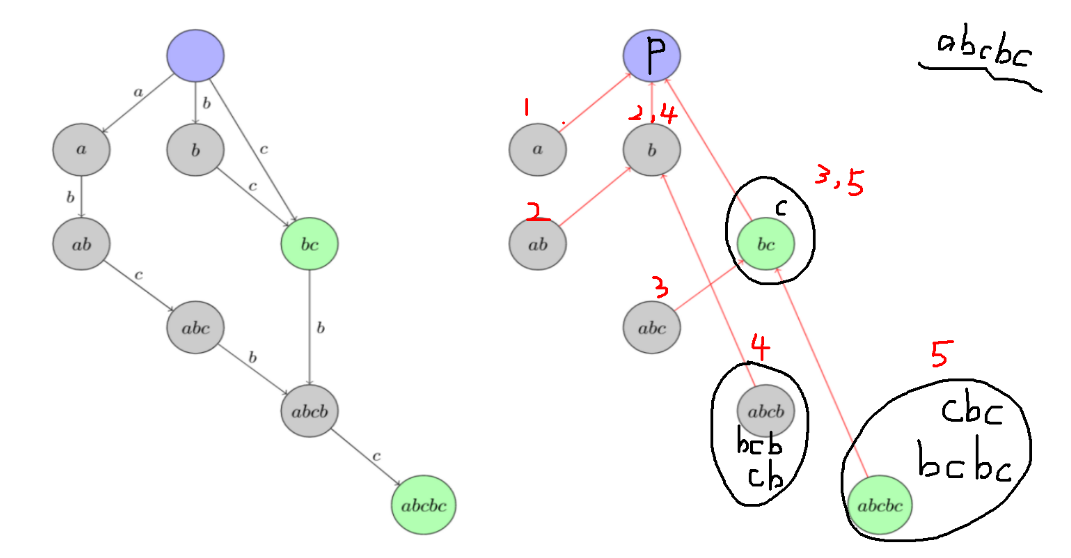
\includegraphics[scale=0.25]{lyh/SAM.png}
    \caption{SAM}
\end{figure}

\subsection{SA}

\begin{lstlisting}[language=C++]
s// 1-based
struct SA {
    int m = 127;
    int n;
    vector<int> sa, rk, height;
    SA(const string &s) {
        n = s.size() - 1;
        sa.resize(n + 1);
        rk.resize(n + 1);
        height.resize(n + 1);
        vector<int> cnt(m + 1);
        for (int i = 1; i <= n; i++) {
            cnt[rk[i] = s[i]]++;
        }
        for (int i = 1; i <= m; i++) {
            cnt[i] += cnt[i - 1];
        }
        for (int i = n; i >= 1; i--) {
            sa[cnt[rk[i]]--] = i;
        }
        vector<int> id(n + 1), oldrk;
        for (int w = 1, p; ; w <<= 1, m = p) {
            int cur = 0;
            for (int i = n - w + 1; i <= n; i++) {
                id[++cur] = i;
            }
            for (int i = 1; i <= n; i++) {
                if (sa[i] > w) {
                    id[++cur] = sa[i] - w;
                }
            }
            cnt.assign(m + 1, 0);
            for (int i = 1; i <= n; i++) {
                cnt[rk[i]]++;
            }
            for (int i = 1; i <= m; i++) {
                cnt[i] += cnt[i - 1];
            }
            for (int i = n; i >= 1; i--) {
                sa[cnt[rk[id[i]]]--] = id[i];
            }
            oldrk = rk;
            p = 0;
            for (int i = 1; i <= n; i++) {
                if (oldrk[sa[i]] == oldrk[sa[i - 1]] && 
                    oldrk[sa[i] + w] == oldrk[sa[i - 1] + w]) {
                    rk[sa[i]] = p;
                } else {
                    rk[sa[i]] = ++p;
                }
            }
            if (p == n) break;
        }
        for (int i = 1, j = 0; i <= n; i++) {
            if (rk[i] == 1) continue;
            if (j) j--;
            while (s[i + j] == s[sa[rk[i] - 1] + j]) {
                j++;
            }
            height[rk[i]] = j;
        }
    }
};

// 应用
int L = 2 * n, K = 20;
vector st(L + 1, vector<int>(K));
for (int i = 1; i <= L; i++) {
    st[i][0] = sa.height[i];
}
for (int j = 1; j < K; j++) {
    for (int i = 1; i + (1 << j) - 1 <= L; i++) {
        st[i][j] = min(st[i][j - 1], st[i + (1 << j - 1)][j - 1]);
    }
}
auto rmq = [&](int l, int r) {
    int k = __lg(r - l + 1);
    return min(st[l][k], st[r - (1 << k) + 1][k]);
};
auto lcp = [&](int i, int j) {
    if (i == j) {
        return n - i + 1;
    }
    int a = sa.rk[i];
    int b = sa.rk[j];
    if (a > b) {
        swap(a, b);
    }
    return rmq(a + 1, b);
};
auto lcs = [&](int i, int j) {
    if (i == j) {
        return i;
    }
    int a = sa.rk[2 * n + 1 - i];
    int b = sa.rk[2 * n + 1 - j];
    if (a > b) {
        swap(a, b);
    }
    return rmq(a + 1, b);
};
// by lyh
\end{lstlisting}

\subsection{SAIS}

\begin{lstlisting}[language=C++]
struct SA {
    vector<int> sa, rk, height;
    SA(const string &init) {
        int n = init.size() - 1;
        vector<int> s;
        for (int i = 1; i <= n; i++) {
            s.push_back(init[i]);
        }
        s.push_back(0);

        sa = SAIS(s, 128);
        rk.assign(n + 1, 0);
        height.assign(n + 1, 0);
        for (int i = 1; i <= n; i++) {
            sa[i]++;
            rk[sa[i]] = i;
        }
        for (int i = 1, j = 0; i <= n; i++) {
            if (rk[i] == 1) continue;
            if (j) j--;
            while (init[i + j] == init[sa[rk[i] - 1] + j]) {
                j++;
            }
            height[rk[i]] = j;
        }
    }
    bool is_LMS_char(const vector<bool> &type, int x) {
        return x >= 1 && type[x] == 1 && type[x - 1] == 0;
    }
    bool is_LMS_equal(const vector<int> &s, vector<bool> &type, int x, int y) {
        do {
            if (s[x] != s[y]) {
                return false;
            }
            x++, y++;
        } while (!is_LMS_char(type, x) && !is_LMS_char(type, y));
        return s[x] == s[y];
    }
    void inducedSort(const vector<int> &s, vector<int> &sa, vector<bool> &type, 
                    vector<int> &bucket, vector<int> &L_bucket, vector<int> &S_bucket, 
                    int ALPHABET_SIZE) {
        int n = s.size() - 1;
        for (int i = 0; i <= n; i++) {
            if (sa[i] > 0) {
                int p = sa[i] - 1;
                if (type[p] == 0) {
                    int ch = s[p];
                    sa[L_bucket[ch]++] = p;
                }
            }
        }
        for (int i = 1; i < ALPHABET_SIZE; i++) {
            S_bucket[i] = bucket[i] - 1;
        }
        for (int i = n; i >= 0; i--) {
            if (sa[i] > 0) {
                int p = sa[i] - 1;
                if (type[p] == 1) {
                    int ch = s[p];
                    sa[S_bucket[ch]--] = p;
                }
            }
        }
    }
    vector<int> SAIS(const vector<int> &s, int ALPHABET_SIZE) {
        int n = s.size() - 1;
        vector<int> bucket(ALPHABET_SIZE, 0);
        vector<int> L_bucket(ALPHABET_SIZE, 0);
        vector<int> S_bucket(ALPHABET_SIZE, 0);
        for (int i = 0; i <= n; i++) {
            bucket[s[i]]++;
        }
        for (int i = 1; i < ALPHABET_SIZE; i++) {
            bucket[i] += bucket[i - 1];
            L_bucket[i] = bucket[i - 1];
            S_bucket[i] = bucket[i] - 1;
        }
        vector<bool> type(n + 1);
        type[n] = 1;  // 终止符是S型 (L: 0, S: 1)
        for (int i = n - 1; i >= 0; i--) {
            if (s[i] < s[i + 1]) {
                type[i] = 1;
            } else if (s[i] > s[i + 1]) {
                type[i] = 0;
            } else {
                type[i] = type[i + 1];
            }
        }
        vector<int> LMS;
        for (int i = 1; i <= n; i++) {
            if (type[i] == 1 && type[i - 1] == 0) {
                LMS.push_back(i);
            }
        }
        int cnt = LMS.size();
        
        vector<int> sa(n + 1, -1);
        for (int i = 0; i < cnt; i++) {
            int ch = s[LMS[i]];
            sa[S_bucket[ch]--] = LMS[i];
        }
        inducedSort(s, sa, type, bucket, L_bucket, S_bucket, ALPHABET_SIZE);
        
        vector<int> name(n + 1, -1);
        int name_cnt = 1, lst = -1;
        bool flag = false;
        for (int i = 1; i <= n; i++) {
            int p = sa[i];
            if (is_LMS_char(type, p)) {
                if (lst >= 0 && !is_LMS_equal(s, type, p, lst)) {
                    name_cnt++;
                }
                if (lst >= 0 && name_cnt == name[lst]) {
                    flag = true;
                }
                name[p] = name_cnt;
                lst = p;
            }
        }
        name[n] = 0;

        vector<int> s1(cnt);
        int pos = 0;
        for (int i = 0; i <= n; i++) {
            if (name[i] >= 0) {
                s1[pos++] = name[i];
            }
        }

        vector<int> sa1;
        if (!flag) {
            sa1.assign(cnt + 1, 0);
            for (int i = 0; i < cnt; i++) {
                sa1[s1[i]] = i;
            }
        } else {
            sa1 = SAIS(s1, name_cnt + 1);
        }
        L_bucket[0] = S_bucket[0] = 0;
        for (int i = 1; i < ALPHABET_SIZE; i++) {
            L_bucket[i] = bucket[i - 1];
            S_bucket[i] = bucket[i] - 1;
        }
        fill(sa.begin(), sa.end(), -1);
        for (int i = cnt - 1; i >= 0; i--) {
            int pos = LMS[sa1[i]];
            int ch = s[pos];
            sa[S_bucket[ch]--] = pos;
        }
        inducedSort(s, sa, type, bucket, L_bucket, S_bucket, ALPHABET_SIZE);
        return sa;
    }
};
\end{lstlisting}

\subsection{PAM}

\begin{lstlisting}[language=C++]
struct PAM {
    constexpr static int ALPHABET_SIZE = 26;
    struct Node {
        int len = 0;
        int link = 0;
        array<int, ALPHABET_SIZE> ch;
        int cnt = 0;
        int dif = 0, slink = 0;
    };
    vector<Node> t;
    int last;
    PAM() {
        init();
    }
    void init() {
        t.assign(2, Node());
        t[1].len = -1;
        t[1].link = -1;
        t[0].link = 1;
        last = 1;
    }
    int newNode() {
        t.emplace_back();
        return t.size() - 1;
    }
    void extend(const string &s, int i) {
        int p = last;
        while (i - t[p].len - 1 < 0 || s[i - t[p].len - 1] != s[i]) {
            p = t[p].link;
        }
        int c = s[i] - 'a';
        if (t[p].ch[c]) {
            last = t[p].ch[c];
        } else {
            int cur = newNode();
            t[cur].len = t[p].len + 2;
            t[p].ch[c] = cur;
            if (p == 1) {
                t[cur].link = 0;
            } else {
                p = t[p].link;
                while (i - t[p].len - 1 < 0 || s[i - t[p].len - 1] != s[i]) {
                    p = t[p].link;
                }
                t[cur].link = t[p].ch[c];
            }
            int pa = t[cur].link;
            t[cur].dif = t[cur].len - t[pa].len;
            if (t[cur].dif == t[pa].dif) {
                t[cur].slink = t[pa].slink;
            } else {
                t[cur].slink = pa;
            }
            last = cur;
        }
        t[last].cnt++;
    }
    Node &operator[](const int &id) {
        return t[id];
    }
};

int g[N], dp[N];

void solve() {
    string s;
    cin >> s;
    int n = s.size();

    string t = "0";
    for (int i = 0; i < n / 2; i++) {
        t += s[i];
        t += s[n - i - 1];
    }

    dp[0] = 1;
    PAM pam;
    for (int i = 1; i <= n; i++) {
        pam.extend(t, i);
        for (int p = pam.last; p > 1; p = pam[p].slink) {
            int sl = pam[p].slink, pa = pam[p].link;
            g[p] = dp[i - pam[sl].len - pam[p].dif];
            if (pam[p].dif == pam[pa].dif) {
                g[p] += g[pa];
                g[p] %= mod;
            }
            if (i % 2 == 0) {
                dp[i] += g[p];
                dp[i] %= mod;
            }
        }
    }

    cout << dp[n] << "\n";
}
\end{lstlisting}

% \begin{figure}
%     \centering
%     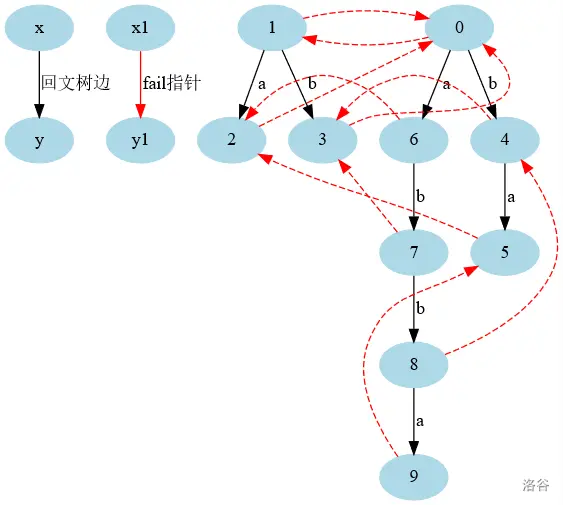
\includegraphics[scale=0.4]{lyh/PAM.png}
%     \caption{PAM}
% \end{figure}

\section{图论}

\subsection{最短路}

\subsubsection{Dijkstra}

\begin{lstlisting}[language=C++]
struct edge {int v, w;};

struct node {
    int dis, u;
    bool operator>(const node& a) const { return dis > a.dis; }
};

vector<edge> e[MAXN];
int dis[MAXN], vis[MAXN];
priority_queue<node, vector<node>, greater<node>> q;

void dijkstra(int n, int s) {
    memset(dis, 0x3f, (n + 1) * sizeof(int));
    memset(vis, 0, (n + 1) * sizeof(int));
    dis[s] = 0;
    q.push({0, s});
    while (!q.empty()) {
        int u = q.top().u;
        q.pop();
        if (vis[u]) continue;
        vis[u] = 1;
        for (auto ed : e[u]) {
            int v = ed.v, w = ed.w;
            if (dis[v] > dis[u] + w) {
                dis[v] = dis[u] + w;
                q.push({dis[v], v});
            }
        }
    }
}
\end{lstlisting}

\subsubsection{Bellman-Ford / SPFA}

可用于判负环

\begin{lstlisting}[language=C++]
struct edge {int v, w;};

vector<edge> e[MAXN];
int dis[MAXN], cnt[MAXN], vis[MAXN];
queue<int> q;

bool spfa(int n, int s) {
    memset(dis, 0x3f, (n + 1) * sizeof(int));
    dis[s] = 0, vis[s] = 1;
    q.push(s);
    while (!q.empty()) {
        int u = q.front();
        q.pop(), vis[u] = 0;
        for (auto ed : e[u]) {
        int v = ed.v, w = ed.w;
        if (dis[v] > dis[u] + w) {
            dis[v] = dis[u] + w;
            cnt[v] = cnt[u] + 1;  // 记录最短路经过的边数
            if (cnt[v] >= n) return false;
            // 在不经过负环的情况下，最短路至多经过 n - 1 条边
            // 因此如果经过了多于 n 条边，一定说明经过了负环
            if (!vis[v]) q.push(v), vis[v] = 1;
        }
        }
    }
    return true;
}
\end{lstlisting}

\subsubsection{Floyd}

\begin{lstlisting}[language=C++]
for (k = 1; k <= n; k++)
    for (x = 1; x <= n; x++)
        for (y = 1; y <= n; y++)
            f[x][y] = min(f[x][y], f[x][k] + f[k][y]);
\end{lstlisting}

判断任意两点之间的连通性，可用 bitset 优化至 $O(n^3/w)$

\begin{lstlisting}[language=C++]
bitset<SIZE> f[SIZE];
for (k = 1; k <= n; k++)
    for (i = 1; i <= n; i++)
        if (f[i][k]) f[i] = f[i] | f[k];
\end{lstlisting}

\subsection{基环树森林的直径}
取环+单调队列求直径. 
\begin{lstlisting}[language=C++]
// 基环树直径的两种可能：a. 不在环上 b. 环的一部分+两条链
#include<bits/stdc++.h>
using namespace std;

using ll = long long;
const int N = 2e6+10;
int n, p, tot = 1, num;
int head[N], nxt[N], ver[N], fa[N], dfn[N], s[N], q[N];
ll edge[N], ps[N], d[N], ans, res;
bool vis[N];

void add(int x, int y, int z){
    ver[++tot] = y; edge[tot] = z;
    nxt[tot] = head[x]; head[x] = tot;
}
void get_cycle(int x, int y, int z){
    ps[1] = z;
    while(y != x){
        s[++p] = y;
        ps[p+1] = edge[fa[y]];
        y = ver[fa[y]^1];
    }
    s[++p] = x;
    for(int i = 1; i <= p; i++){
        vis[s[i]] = 1;
        s[i+p] = s[i];
        ps[i+p] = ps[i];
    }
    for(int i = 1; i <= 2*p; i++)
        ps[i] += ps[i-1];
}
void dp(int x){
    vis[x] = 1;
    for(int i = head[x]; i; i = nxt[i]){
        int y = ver[i], z = edge[i];
        if(vis[y]) continue;
        dp(y);
        ans = max(ans, d[x]+d[y]+z);
        d[x] = max(d[x], d[y]+z);
    }
}
void dfs(int x){
    dfn[x] = ++num;
    for(int i = head[x]; i; i = nxt[i]){
        int y = ver[i], z = edge[i];
        if(!dfn[y]){
            fa[y] = i;
            dfs(y);
        }
        else if((i^1) != fa[x] && dfn[y] > dfn[x]){
            get_cycle(x, y, z);
        }
    }
}
int main(){
    ios::sync_with_stdio(0);
    cin >> n;
    for(int x = 1; x <= n; x++){
        int y, z; cin >> y >> z;
        add(x, y, z); add(y, x, z);
    }
    for(int i = 1; i <= n; i++) if(!dfn[i]){
        p = 0; ans = 0;
        dfs(i);
        for(int j = 1; j <= p; j++) dp(s[j]);
        int l = 1, r = 0;
        for(int j = 1; j <= 2*p; j++){
            while(l <= r && j-q[l] >= p) l++;
            if(l <= r) ans = max(ans, d[s[j]]+d[s[q[l]]]+ps[j]-ps[q[l]]);
            while(l <= r && d[s[q[r]]]-ps[q[r]] <= d[s[j]]-ps[j]) r--;
            q[++r] = j; 
        }
        res += ans;
    }
    cout << res << endl;
    return 0;
}
\end{lstlisting}

\subsection{树链剖分}
轻重链剖分
\begin{lstlisting}[language=C++]
struct HLD {
    int n;
    vector<vector<int>> adj;
    vector<int> dep, siz, parent, in, out, ord, top;
    int cur;

    HLD(int n) {
        init(n);
    }
    void init(int n) {
        this->n = n;
        adj.assign(n, {});
        dep.resize(n);
        siz.resize(n);
        parent.resize(n);
        in.resize(n);
        out.resize(n);
        ord.resize(n);
        top.resize(n);
        cur = 0;
    }
    void addEdge(int u, int v) {
        adj[u].push_back(v);
        adj[v].push_back(u);
    }
    void work(int root) {
        top[root] = root;
        dep[root] = 1;
        parent[root] = 0;
        dfs1(root, 0);
        dfs2(root, 0);
    }
    void dfs1(int u, int pa) {
        siz[u] = 1;
        for (auto &v : adj[u]) {
            if (v == pa) {
                continue;
            }
            parent[v] = u;
            dep[v] = dep[u] + 1;
            dfs1(v, u);
            siz[u] += siz[v];
            if (siz[v] > siz[adj[u][0]]) {
                swap(v, adj[u][0]);
            }
        }
    }
    void dfs2(int u, int pa) {
        in[u] = ++cur;
        ord[in[u]] = u;
        for (auto v : adj[u]) {
            if (v == pa) {
                continue;
            }
            top[v] = (v == adj[u][0] ? top[u] : v);
            dfs2(v, u);
        }
        out[u] = cur;
    }
    int lca(int u, int v) {
        while (top[u] != top[v]) {
            if (dep[top[u]] > dep[top[v]]) {
                swap(u, v);
            }
            v = parent[top[v]];
        }
        return dep[u] > dep[v] ? v : u;
    }
};

// 路径修改
auto pathModify = [&](int u, int v, int k) {
    while (t.top[u] != t.top[v]) {
        if (t.dep[t.top[u]] > t.dep[t.top[v]]) {
            swap(u, v);
        }
        seg.rangeModify(t.in[t.top[v]], t.in[v], {k});
        v = t.parent[t.top[v]];
    }
    if (t.dep[u] > t.dep[v]) {
        swap(u, v);
    }
    seg.rangeModify(t.in[u], t.in[v], {k});
};

// 路径查询
auto pathQuery = [&](int u, int v) {
    int res = 0;
    while (t.top[u] != t.top[v]) {
        if (t.dep[t.top[u]] > t.dep[t.top[v]]) {
            swap(u, v);
        }
        res += seg.rangeQuery(t.in[t.top[v]], t.in[v]).sum, res %= mod;
        v = t.parent[t.top[v]];
    }
    if (t.dep[u] > t.dep[v]) {
        swap(u, v);
    }
    res += seg.rangeQuery(t.in[u], t.in[v]).sum, res %= mod;
    return res;
};

// 子树修改
auto subtreeModify = [&](int u, int k) {
    seg.rangeModify(t.in[u], t.out[u], {k});
};

// 子树查询
auto subtreeQuery = [&](int u) {
    return seg.rangeQuery(t.in[u], t.out[u]).sum % mod;
};
// by lyh
\end{lstlisting}

\subsection{LCA}

\subsection{无向图连通性}

\subsubsection{割点和桥}

割点判定法则：
\[dfn[x]\le low[y]\]
其中 $low[y]$ 表示 \underline{子树}以及 \underline{通过一条非搜索树上的边能够到达的子树外的点} 的最小 $dfn$。特别地，对于根节点，要有两个点满足上述条件。由于是小于等于，父亲节点实际上可取。
\begin{lstlisting}[language=C++]
void Tarjan(int u, int pa) {
    low[u] = dfn[u] = ++dfn_cnt;
    for (auto v : adj[u]) {
        if (v == pa) continue;
        if (!dfn[v]) {
            if (pa == 0) {
                son_cnt++; // 若u是搜索起点, 更新儿子数量
            }
            Tarjan(v, u);
            low[u] = min(low[u], low[v]);

            if (pa != 0 && low[v] >= dfn[u] && !is_cut[u]) { 
                cut_cnt++;
                is_cut[u] = true;
            }
        } else {
            low[u] = min(low[u], dfn[v]); 
        }
    }
    if (pa == 0 && son_cnt >= 2 && !is_cut[u]) { // 搜索起点有两个及以上的儿子
        cut_cnt++;
        is_cut[u] = true;
    }
}
//by lyh
\end{lstlisting}

\begin{lstlisting}[language=C++]
void tarjan(int x){
    dfn[x] = low[x] = ++tot;
    int cnt = 0;
    for(auto y: e[x]) if(!dfn[y]){
        tarjan(y);
        low[x] = min(low[x], low[y]);
        if(dfn[x] <= low[y]){
            ++cnt;
            if(x != root || cnt > 1) cut[x] = 1;
        }
    }
    else low[x] = min(low[x], dfn[y]);
}
// if(!dfn[x]) root = x, tarjan(x);
// by zzy
\end{lstlisting}

割边判定法则：
\[dfn[x]< low[y]\]
父亲节点不可取，注意特判有重边的情况。
\begin{lstlisting}[language=C++]
void Tarjan(int u, int lst) {
    low[u] = dfn[u] = ++dfn_cnt;
    for (auto [v, id] : adj[u]) {
        if (id == lst) {
            continue;
        }
        if (!dfn[v]) {
            Tarjan(v, id);
            low[u] = min(low[u], low[v]);
            
            if (low[v] > dfn[u]) {
                bridge_cnt++;
                is_bridge[id] = true;
            }
        } else {
            low[u] = min(low[u], dfn[v]);
        }
    }
}
// by lyh
\end{lstlisting}

\subsubsection{e-DCC 和 v-DCC}

边双连通分量
\begin{lstlisting}[language=C++]
struct EBCC {
    int n;
    vector<vector<array<int, 2>>> adj;
    vector<int> stk;
    vector<int> dfn, low, bel;
    int cur, cnt;

    EBCC(int n) {
        init(n);
    }
    void init(int n) {
        this->n = n;
        adj.assign(n, {});
        dfn.assign(n, 0);
        low.resize(n);
        bel.assign(n, 0);
        stk.clear();
        cur = cnt = 0;
    }
    void addEdge(int u, int v, int id) {
        adj[u].push_back({v, id});
        adj[v].push_back({u, id});
    }
    void Tarjan(int u, int lst) {
        dfn[u] = low[u] = ++cur;
        stk.push_back(u);

        for (auto [v, id] : adj[u]) {
            if (id == lst) {
                continue;
            }
            if (!dfn[v]) {
                Tarjan(v, id);
                low[u] = min(low[u], low[v]);
            } else {
                low[u] = min(low[u], dfn[v]);
            }
        }

        if (low[u] == dfn[u]) {
            cnt++;
            int v;
            do {
                v = stk.back();
                stk.pop_back();
                bel[v] = cnt;
            } while (v != u);
        }
    }
    vector<int> work() {
        for (int i = 1; i < n; i++) {
            if (!dfn[i]) {
                Tarjan(i, 0);
            }
        }
        return bel;
    }
};
\end{lstlisting}

点双连通分量
\begin{lstlisting}[language=C++]
struct VBCC {
    int n;
    vector<vector<int>> adj;
    vector<int> stk;
    vector<int> dfn, low;
    int cur, cnt;

    VBCC(int n) {
        init(n);
    }
    void init(int n) {
        this->n = n;
        adj.assign(n, {});
        dfn.assign(n, 0);
        low.resize(n);
        cur = cnt = 0;
    }
    void addEdge(int u, int v) {
        adj[u].push_back(v);
        adj[v].push_back(u);
    }
    void Tarjan(int u, int pa) {
        dfn[u] = low[u] = ++cur;
        stk.push_back(u);
        
        for (auto v : adj[u]) {
            if (v == pa) {
                continue;
            }
            if (!dfn[v]) {
                Tarjan(v, u);
                low[u] = min(low[u], low[v]);

                if (low[v] >= dfn[u]) {
                    vbcc.emplace_back();
                    cnt++;
                    int y;
                    do {
                        y = stk.back();
                        stk.pop_back();
                        vbcc[cnt].push_back(y);
                    } while (y != v);
                    vbcc[cnt].push_back(u);
                }
            } else {
                low[u] = min(low[u], dfn[v]);
            }
        }

        if (pa == 0 && adj[u].size() == 0) {
            vbcc.emplace_back();
            cnt++;
            vbcc[cnt].push_back(u);
        }
    }
    auto work() {
        for (int i = 1; i < n; i++) {
            if (!dfn[i]) {
                Tarjan(i, 0);
            }
        }
        return vbcc;
    }
};
// by lyh
\end{lstlisting}

\subsection{有向图连通性}

Tarjan求强连通分量
\begin{lstlisting}[language=C++]
struct SCC {
    int n;
    vector<vector<int>> adj;
    vector<int> stk;
    vector<int> dfn, low, bel;
    int cur, cnt;
    
    SCC(int n) {
        init(n);
    }
    void init(int n) {
        this->n = n;
        adj.assign(n, {});
        dfn.assign(n, 0);
        low.resize(n);
        bel.assign(n, 0);
        stk.clear();
        cur = cnt = 0;
    }
    void addEdge(int u, int v) {
        adj[u].push_back(v);
    }
    void Tarjan(int u) {
        dfn[u] = low[u] = ++cur;
        stk.push_back(u);
        
        for (auto v : adj[u]) {
            if (!dfn[v]) {
                Tarjan(v);
                low[u] = min(low[u], low[v]);
            } else if (!bel[v]) {
                low[u] = min(low[u], dfn[v]);
            }
        }
        
        if (dfn[u] == low[u]) {
            cnt++;
            int v;
            do {
                v = stk.back();
                stk.pop_back();
                bel[v] = cnt;
            } while (v != u);
        }
    }
    vector<int> work() {
        for (int i = 1; i < n; i++) {
            if (!dfn[i]) {
                Tarjan(i);
            }
        }
        return bel;
    }
};
// by lyh
\end{lstlisting}

\subsection{欧拉回路}
有向图版本
\begin{lstlisting}[language=C++]
void solve() {
    int n, m;
    cin >> n >> m;
    vector<vector<int>> e(n + 1);
    vector<int> in(n + 1), out(n + 1);
    for (int i = 1; i <= m; i++) {
        int u, v;
        cin >> u >> v;
        e[u].push_back(v);
        out[u]++;
        in[v]++;
    }
    
    int cnt1 = 0, cnt2 = 0, s = 1;
    for (int i = 1; i <= n; i++) {
        sort(e[i].begin(), e[i].end());
        if (out[i] != in[i]) {
            if (out[i] == in[i] + 1) {
                cnt1++;
                s = i;
            } else if (out[i] + 1 == in[i]) {
                cnt2++;
            } else {
                cout << "No\n";
                return;
            }
        }
    }
    if (!(cnt1 == 1 && cnt2 == 1 || cnt1 == 0 && cnt2 == 0)) {
        cout << "No\n";
        return;
    }

    vector<int> cur(n + 1);
    stack<int> st;
    auto dfs = [&](auto self, int u) -> void {
        for (int i = cur[u]; i < e[u].size(); i = cur[u]) {
            cur[u] = i + 1;
            int v = e[u][i];
            self(self, v);
        }
        st.push(u);
    };
    dfs(dfs, s);

    while (st.size()) {
        cout << st.top() << " ";
        st.pop();
    }
}
\end{lstlisting}
无向图版本
\begin{lstlisting}[language=C++]
void solve() {
    int n = 500, m;
    cin >> m;
    vector<vector<array<int, 2>>> e(n + 1);
    vector<int> d(n + 1);
    int s = n;
    for (int i = 1; i <= m; i++) {
        int u, v;
        cin >> u >> v;
        e[u].push_back({v, i});
        e[v].push_back({u, i});
        d[u]++;
        d[v]++;
        s = min(s, min(u, v));
    }
    
    for (int i = n; i >= 1; i--) {
        sort(e[i].begin(), e[i].end());
        if (d[i] % 2 == 1) {
            s = i;
        }
    }

    vector<bool> vis(m + 1);
    vector<int> cur(n + 1);
    stack<int> st;
    auto dfs = [&](auto &&self, int u) -> void {
        for (int &j = cur[u]; j < e[u].size(); j++) {
            auto [v, i] = e[u][j];
            if (!vis[i]) {
                vis[i] = true;
                self(self, v);
                // ans.push_back(i);
            }
        }
        st.push(u);
    };
    dfs(dfs, s);

    while (st.size()) {
        cout << st.top() << "\n";
        st.pop();
    }
}
\end{lstlisting}
\subsection{二分图}

\subsection{网络流}

\subsubsection{最大流}

\begin{lstlisting}[language=C++]
template<class T>
struct MaxFlow {
    struct _Edge {
        int to;
        T cap;
    };
    int n;
    vector<_Edge> e;
    vector<vector<int>> g;
    vector<int> cur, h;
    MaxFlow(int n) {
        init(n);
    }
    void init(int n) {
        this->n = n;
        e.clear();
        g.assign(n, {});
        cur.resize(n);
        h.resize(n);
    }
    bool bfs(int s, int t) {
        h.assign(n, -1);
        queue<int> q;
        h[s] = 0;
        q.push(s);
        while (!q.empty()) {
            auto u = q.front();
            q.pop();
            for (auto i : g[u]) {
                auto [v, c] = e[i];
                if (c > 0 && h[v] == -1) {
                    h[v] = h[u] + 1;
                    if (v == t) {
                        return true;
                    }
                    q.push(v);
                }
            }
        }
        return false;
    }
    T dfs(int u, int t, T f) {
        if (u == t) {
            return f;
        }
        auto r = f;
        for (int &i = cur[u]; i < int(g[u].size()); i++) {
            auto j = g[u][i];
            auto [v, c] = e[j];
            if (c > 0 && h[v] == h[u] + 1) {
                auto a = dfs(v, t, min(r, c));
                e[j].cap -= a;
                e[j ^ 1].cap += a;
                r -= a;
                if (r == 0) {
                    return f;
                }
            }
        }
        return f - r;
    }
    void addEdge(int u, int v, T cap) {
        g[u].push_back(e.size());
        e.push_back({v, cap});
        g[v].push_back(e.size());
        e.push_back({u, 0});
    }
    T flow(int s, int t) {
        T ans = 0;
        while (bfs(s, t)) {
            cur.assign(n, 0);
            ans += dfs(s, t, inf);
        }
        return ans;
    }
    vector<bool> minCut() {
        vector<bool> c(n);
        for (int i = 0; i < n; i++) {
            c[i] = (h[i] != -1);
        }
        return c;
    }
    struct Edge {
        int from;
        int to;
        T cap;
        T flow;
    };
    vector<Edge> edges() {
        vector<Edge> res;
        for (int i = 0; i < e.size(); i += 2) {
            res.push_back({e[i + 1].to, e[i].to, e[i].cap + e[i + 1].cap, e[i + 1].cap});
        }
        return res;
    }
};
// by lyh
\end{lstlisting}

\subsubsection{最小费用最大流}

\begin{lstlisting}[language=C++]
template<class T>
struct MinCostFlow {
    struct _Edge {
        int to;
        T cap;
        T cost;
    };
    int n;
    vector<_Edge> e;
    vector<vector<int>> g;
    vector<T> h, dis;
    vector<int> pre;
    bool Dijkstra(int s, int t) {
        dis.assign(n, inf);
        pre.assign(n, -1);
        priority_queue<pair<T, int>, vector<pair<T, int>>, greater<pair<T, int>>> q;
        dis[s] = 0;
        q.push({0, s});
        while (!q.empty()) {
            auto [d, u] = q.top();
            q.pop();
            if (dis[u] < d) {
                continue;
            }
            for (auto id : g[u]) {
                auto [v, cap, cost] = e[id];
                if (cap > 0 && dis[v] > d + h[u] - h[v] + cost) {
                    dis[v] = d + h[u] - h[v] + cost;
                    pre[v] = id;
                    q.push({dis[v], v});
                }
            }
        }
        return dis[t] != inf;
    }
    MinCostFlow() {}
    MinCostFlow(int n_) {
        init(n_);
    }
    void init(int n_) {
        n = n_;
        e.clear();
        g.assign(n, {});
    }
    void addEdge(int u, int v, T cap, T cost) {
        g[u].push_back(e.size());
        e.push_back({v, cap, cost});
        g[v].push_back(e.size());
        e.push_back({u, 0, -cost});
    }
    pair<T, T> flow(int s, int t) {
        T flow = 0, cost = 0;
        h.assign(n, 0);
        while (Dijkstra(s, t)) {
            for (int i = 0; i < n; i++) {
                h[i] += dis[i];
            }
            T aug = inf;
            for (int i = t; i != s; i = e[pre[i] ^ 1].to) {
                aug = min(aug, e[pre[i]].cap);
            }
            for (int i = t; i != s; i = e[pre[i] ^ 1].to) {
                e[pre[i]].cap -= aug;
                e[pre[i] ^ 1].cap += aug;
            }
            flow += aug;
            cost += aug * h[t];
        }
        return {flow, cost};
    }
    struct Edge {
        int from;
        int to;
        T cap;
        T cost;
        T flow;
    };
    vector<Edge> edges() {
        vector<Edge> res;
        for (int i = 0; i < e.size(); i += 2) {
            Edge ed = {e[i + 1].to, e[i].to, e[i].cap + e[i + 1].cap, e[i].cost, e[i + 1].cap};
            res.push_back(ed);
        }
        return res;
    }
};
// by lyh
\end{lstlisting}

\section{计算几何}

\subsection{Point \& Line}

\begin{lstlisting}[language=C++]
using i128 = __int128_t;
using ld = double;
constexpr ld PI = 3.1415926535;
constexpr ld EPS = 1e-6;

template<class T>
struct Point {
    T x, y;
    Point(const T &x_ = 0, const T &y_ = 0) : x(x_), y(y_) {}
    
    template<class U>
    operator Point<U>() {
        return Point<U>(U(x), U(y));
    }
    friend Point operator+(const Point &a, const Point &b) {
        return Point(a.x + b.x, a.y + b.y);
    }
    friend Point operator-(const Point &a, const Point &b) {
        return Point(a.x - b.x, a.y - b.y);
    }
    friend Point<ld> operator*(const Point &a, ld t) {
        return Point<ld>(a.x * t, a.y * t);
    }
    friend Point<ld> operator/(const Point &a, ld t) {
        return Point<ld>(a.x / t, a.y / t);
    }
    friend bool operator==(const Point &a, const Point &b) {
        return a.x == b.x && a.y == b.y;
    }
    friend istream &operator>>(istream &is, Point &a) {
        return is >> a.x >> a.y;
    }
    friend ostream &operator<<(ostream &os, const Point &a) {
        return os << "(" << a.x << ", " << a.y << ")";
    }
};

template<class T>
T dot(const Point<T> &a, const Point<T> &b) {
    return a.x * b.x + a.y * b.y;
}

template<class T>
T cross(const Point<T> &a, const Point<T> &b) {
    return a.x * b.y - a.y * b.x;
}

template<class T>
struct Line {
    Point<T> a, b;
    Line(const Point<T> &a_ = Point<T>(), const Point<T> &b_ = Point<T>()) : a(a_), b(b_) {}
};

# Point
// p以p0为中心逆时针旋转a
template<class T>
Point<ld> rotate(const Point<T> &p, const Point<T> &p0, ld a) {
    return {
        (p.x - p0.x) * cosl(a) - (p.y - p0.y) * sinl(a) + p0.x, 
        (p.y - p0.y) * cosl(a) + (p.x - p0.x) * sinl(a) + p0.y
    };
}

# Line
template<class T>
bool parallel(const Line<T> &l1, const Line<T> &l2) {
    return cross(l1.b - l1.a, l2.b - l2.a) == 0;
}

// 线段l1, l2是否相交
template<class T>
bool is_SS_Intersect(const Line<T> &l1, const Line<T> &l2) {
    if (cross(l1.b - l1.a, l2.a - l1.a) * cross(l1.b - l1.a, l2.b - l1.a) > 0) return false;
    if (cross(l2.b - l2.a, l1.a - l2.a) * cross(l2.b - l2.a, l1.b - l2.a) > 0) return false;
    return true;
}

// 直线l1和线段l2是否相交
template<class T>
bool is_LS_Intersect(const Line<T> &l1, const Line<T> &l2) {
    return cross(l1.b - l1.a, l2.a - l1.a) * cross(l1.b - l1.a, l2.b - l1.a) <= 0;
}

// 求直线l1, l2的交点a + ut, t = (a - b) ^ v / (v ^ u)
template<class T>
Point<ld> lineIntersection(const Line<T> &l1, const Line<T> &l2) {
    Point<ld> u(l1.b - l1.a), v(l2.b - l2.a);
    return Point<ld>(l1.a) + u * (cross(Point<ld>(l1.a - l2.a), v) / cross(v, u));
}

# PL
template<class T>
ld distancePL(const Point<T> &p, const Line<T> &l) {
    return abs(cross(l.b - l.a, l.b - p)) / length(l);
}

template<class T>
ld distancePS(const Point<T> &p, const Line<T> &l) {
    if (dot(p - l.a, l.b - l.a) < 0) {
        return distance(p, l.a);
    }
    if (dot(p - l.b, l.a - l.b) < 0) {
        return distance(p, l.b);
    }
    return distancePL(p, l);
}

template<class T>
bool pointOnLineLeft(const Point<T> &p, const Line<T> &l) {
    return cross(l.b - l.a, p - l.a) > 0;
}

template<class T>
bool pointOnSegment(const Point<T> &p, const Line<T> &l) {
    return cross(p - l.a, l.b - l.a) == 0 
    && min(l.a.x, l.b.x) <= p.x && p.x <= max(l.a.x, l.b.x)
    && min(l.a.y, l.b.y) <= p.y && p.y <= max(l.a.y, l.b.y);
}
\end{lstlisting}

\subsection{Polygon}

\begin{lstlisting}[language=C++]
// 多边形有向面积的2倍，注意是否要开__int128_t
template<class T>
T directedArea(const vector<Point<T>> &p) {
    int n = p.size();
    T res = 0;
    for (int i = 0; i < n; i++) {
        auto u = p[(i + 1) % n] - p[i];
        auto v = p[0] - p[i];
        res += cross(u, v);
    }
    return res;
}

// 判断多边形逆时针给出(1)还是顺时针给出(0)，另一种判断方法是极点
template<class T>
bool isCounterClockwise(const vector<Point<T>> &p) {
    return directedArea(p) > 0;
}

template<class T>
bool pointInPolygon(const Point<T> &A, const vector<Point<T>> &p) {
    int n = p.size();
    for (int i = 0; i < n; i++) {
        auto u = p[(i + 1) % n] - p[i];
        auto v = a - p[i];
        if (cross(u, v) < 0) {
            return false;
        }
    }
    return true;
}

vector<P> stk;
void Andrew(vector<P> p) {
    stk.clear();
    sort(p.begin(), p.end(), [&](P A, P B) {
        return A.x != B.x ? A.x < B.x : A.y < B.y;
    });
    int n = p.size();
    for (int i = 0; i < n; i++) {
        int top = stk.size();
        while (top >= 2 && cross(stk[top - 1] - stk[top - 2], p[i] - stk[top - 2]) <= 0) {
            top--;
            stk.pop_back();
        }
        stk.push_back(p[i]);
    }
    int top1 = stk.size();
    for (int i = n - 1; i >= 0; i--) {
        int top = stk.size();
        while (top > top1 && cross(stk[top - 1] - stk[top - 2], p[i] - stk[top - 2]) <= 0) {
            top--;
            stk.pop_back();
        }
        stk.push_back(p[i]);
    }
}
\end{lstlisting}

\subsection{半平面交}

\begin{lstlisting}[language=C++]
template<class T>
int sgn(const Point<T> &p) {
    return p.y > 0 || (p.y == 0 && p.x > 0) ? 1 : -1;
}

template<class T>
bool pointOnLineLeft(const Point<T> &p, const Line<T> &l) {
    return cross(l.b - l.a, p - l.a) > 0;
}

// 求直线l1, l2的交点a + ut, t = (a - b) ^ v / (v ^ u)
template<class T>
Point<ld> lineIntersection(const Line<T> &l1, const Line<T> &l2) {
    Point<ld> u(l1.b - l1.a), v(l2.b - l2.a);
    return Point<ld>(l1.a) + u * (cross(Point<ld>(l1.a - l2.a), v) / cross(v, u));
}

template<class T>
vector<Point<T>> hp(vector<Line<T>> lines) {
    sort(lines.begin(), lines.end(), [&](auto l1, auto l2) {
        auto d1 = l1.b - l1.a;
        auto d2 = l2.b - l2.a;
        if (sgn(d1) != sgn(d2)) {
            return sgn(d1) == 1;
        }
        return cross(d1, d2) > 0;
    });
    
    deque<Line<T>> ls;
    deque<Point<T>> ps;
    for (auto l : lines) {
        if (ls.empty()) {
            ls.push_back(l);
            continue;
        }
        while (!ps.empty() && !pointOnLineLeft(ps.back(), l)) {
            ps.pop_back();
            ls.pop_back();
        }
        while (!ps.empty() && !pointOnLineLeft(ps[0], l)) {
            ps.pop_front();
            ls.pop_front();
        }
        if (cross(l.b - l.a, ls.back().b - ls.back().a) == 0) {
            if (dot(l.b - l.a, ls.back().b - ls.back().a) > 0) {
                if (!pointOnLineLeft(ls.back().a, l)) {
                    assert(ls.size() == 1);
                    ls[0] = l;
                }
                continue;
            }
            return {};
        }
        ps.push_back(lineIntersection(ls.back(), l));
        ls.push_back(l);
    }

    while (!ps.empty() && !pointOnLineLeft(ps.back(), ls[0])) {
        ps.pop_back();
        ls.pop_back();
    }
    if (ls.size() <= 2) {
        return {};
    }
    ps.push_back(lineIntersection(ls[0], ls.back()));
    
    return vector(ps.begin(), ps.end());
}
\end{lstlisting}

\subsection{最小圆覆盖}
\begin{lstlisting}[language=C++]
template<class T>
struct Circle {
    Point<T> c;
    T r;
    Circle(Point<T> c_, T r_ = -1) : c(c_), r(r_) {}
};

using P = Point<ld>;
using C = Circle<ld>;

mt19937_64 rng(chrono::steady_clock::now().time_since_epoch().count());

Circle<ld> CircleFrom3(P a, P b, P c) {
    ld D = 2 * (a.x * (b.y - c.y) + b.x * (c.y - a.y) + c.x * (a.y - b.y));
    if (abs(D) < EPS) {
        ld d01 = distance(a, b), d02 = distance(a, c), d12 = distance(b, c);
        if (d02 <= d01 && d12 <= d01) {
            return Circle(Point<ld>(a + b) / 2.0, d01 / 2.0);
        } else if (d01 <= d02 && d12 <= d02) {
            return Circle(Point<ld>(a + c) / 2.0, d02 / 2.0);
        } else {
            return Circle(Point<ld>(b + c) / 2.0, d12 / 2.0);
        }
    }
    ld da = dot(a, a), db = dot(b, b), dc = dot(c, c);
    Point<ld> center(0, 0);
    center.x = 1.0 * (da * (b.y - c.y) + db * (c.y - a.y) + dc * (a.y - b.y)) / D;
    center.y = 1.0 * (da * (c.x - b.x) + db * (a.x - c.x) + dc * (b.x - a.x)) / D;
    ld radius = distance<ld>(center, a);
    return Circle(center, radius);
}
Circle<ld> MinimumEnclosingCircle(vector<P> &p) {
    int n = p.size();
    if (n == 0) {
        return {{0, 0}, -1};
    } else if (n == 1) {
        return {p[0], 0};
    }
    shuffle(p.begin(), p.end(), rng);
    Circle<ld> mec = {Point<ld>(p[0] + p[1]) / 2.0, distance<ld>(p[0], p[1]) / 2.0};
    for (int i = 2; i < n; i++) {
        if (square(Point<ld>(p[i]) - mec.c) < mec.r * mec.r + EPS) {
            continue;
        }
        mec = {Point<ld>(p[0] + p[i]) / 2.0, distance<ld>(p[0], p[i]) / 2.0};
        for (int j = 1; j < i; j++) {
            if (square(Point<ld>(p[j]) - mec.c) < mec.r * mec.r + EPS) {
                continue;
            }
            mec = {Point<ld>(p[i] + p[j]) / 2.0, distance<ld>(p[i], p[j]) / 2.0};
            for (int k = 0; k < j; k++) {
                if (square(Point<ld>(p[k]) - mec.c) < mec.r * mec.r + EPS) {
                    continue;
                }
                mec = CircleFrom3(p[i], p[j], p[k]);
            }
        }
    }
    return mec;
}
\end{lstlisting}

\subsection{三维计算几何}

\begin{lstlisting}[language=C++]
using ld = double;
struct Point {
    ld x, y, z;
    Point(const ld &x_ = 0, const ld &y_ = 0, const ld &z_ = 0) : x(x_), y(y_), z(z_) {}

    friend Point operator+(const Point &a, const Point &b) {
        return {a.x + b.x, a.y + b.y, a.z + b.z};
    }
    friend Point operator-(const Point &a, const Point &b) {
        return {a.x - b.x, a.y - b.y, a.z - b.z};
    }
    friend Point operator*(const Point &a, ld k) {
        return {a.x * k, a.y * k, a.z * k};
    }
    friend Point operator/(const Point &a, ld k) {
        return {a.x / k, a.y / k, a.z / k};
    }
};

Point cross(const Point &a, const Point &b) {
    return {
        a.y * b.z - a.z * b.y,
        a.z * b.x - a.x * b.z,
        a.x * b.y - a.y * b.x
    };
}

ld dot(const Point &a, const Point &b) {
    return a.x * b.x + a.y * b.y + a.z * b.z;
}

ld length(const Point &a) {
    return sqrtl(dot(a, a));
}

Point normalize(const Point &a) {
    return a / length(a);
}

// 向量p在点p0和法向量f确定的平面上的投影向量
Point projectOnPlane(const Point &p, const Point &p0, const Point &f) {
    auto a = p - p0;
    auto a0 = f * dot(a, f) / dot(f, f); // a在f上的投影
    return a - a0;
}

// 投影向量p在p0为原点，向量u, v为x, y轴的平面上的坐标
array<ld, 2> pointOnPlane(const Point &p, const Point &p0, const Point &u, const Point &v) {
    auto a = p - p0;
    ld x = dot(a, u);
    ld y = dot(a, v);
    return {x, y};
}
\end{lstlisting}

\end{document}